\documentclass[a4paper,12pt, oneside]{book}

% \usepackage{fullpage}
\usepackage[italian]{babel}
\usepackage[utf8]{inputenc}
\usepackage{amssymb}
\usepackage{amsthm}
\usepackage{graphics}
\usepackage{amsfonts}
\usepackage{listings}
\usepackage{amsmath}
\usepackage{amstext}
\usepackage{engrec}
\usepackage{rotating}
\usepackage{verbatim}
\usepackage[safe,extra]{tipa}
\usepackage{showkeys}
\usepackage{multirow}
\usepackage{hyperref}
\usepackage{microtype}
\usepackage{fontspec}
\usepackage{enumerate}
\usepackage{braket}
\usepackage{marginnote}
\usepackage{pgfplots}
\usepackage{cancel}
\usepackage{polynom}
\usepackage{booktabs}
\usepackage{enumitem}
\usepackage{framed}
\usepackage{pdfpages}
\usepackage{pgfplots}
\usepackage{algorithm}
% \usepackage{algpseudocode}
\usepackage[cache=false]{minted}
\usepackage{mathtools}
\usepackage[noend]{algpseudocode}
\usepackage{tikz}\usetikzlibrary{er}\tikzset{multi  attribute /.style={attribute ,double  distance =1.5pt}}\tikzset{derived  attribute /.style={attribute ,dashed}}\tikzset{total /.style={double  distance =1.5pt}}\tikzset{every  entity /.style={draw=orange , fill=orange!20}}\tikzset{every  attribute /.style={draw=MediumPurple1, fill=MediumPurple1!20}}\tikzset{every  relationship /.style={draw=Chartreuse2, fill=Chartreuse2!20}}\newcommand{\key}[1]{\underline{#1}}


\usepackage{fancyhdr}
\pagestyle{fancy}
\fancyhead[LE,RO]{\slshape \rightmark}
\fancyhead[LO,RE]{\slshape \leftmark}
\fancyfoot[C]{\thepage}


\title{Analisi e Progetto di Algoritmi}
\author{UniShare\\\\Davide Cozzi\\\href{https://t.me/dlcgold}{@dlcgold}\\\\Gabriele De Rosa\\\href{https://t.me/derogab}{@derogab} \\\\Federica Di Lauro\\\href{https://t.me/f_dila}{@f\textunderscore dila}}
\date{}

\pgfplotsset{compat=1.13}
\begin{document}
\maketitle

\definecolor{shadecolor}{gray}{0.80}
\setlist{leftmargin = 2cm}
\newtheorem{teorema}{Teorema}
\newtheorem{definizione}{Definizione}
\newtheorem{esempio}{Esempio}
\newtheorem{corollario}{Corollario}
\newtheorem{lemma}{Lemma}
\newtheorem{osservazione}{Osservazione}
\newtheorem{nota}{Nota}
\newtheorem{esercizio}{Esercizio}
\algdef{SE}[DOWHILE]{Do}{doWhile}{\algorithmicdo}[1]{\algorithmicwhile\ #1}
\tableofcontents
\renewcommand{\chaptermark}[1]{%
  \markboth{\chaptername
    \ \thechapter.\ #1}{}}
\renewcommand{\sectionmark}[1]{\markright{\thesection.\ #1}}
\newcommand{\floor}[1]{\lfloor #1 \rfloor}

\chapter{Introduzione}
\textbf{Questi appunti sono presi a lezione. Per quanto sia stata fatta una revisione è altamente probabile (praticamente certo) che possano contenere errori, sia di stampa che di vero e proprio contenuto. Per eventuali proposte di correzione effettuare una pull request. Link: } \url{https://github.com/dlcgold/Appunti}.\\
\textbf{Grazie mille e buono studio!}
\\
\begin{comment}

  \begin{algorithm}
    \If {$i \gets 1$}
    \State $test$
    \Else
    \State $bho$
    \EndIf
    \While {$test$}
    \State $cose$
    \EndWhile
    \For {$cose...$}
    \State $altre cose$
    \EndFor

    \Function{Increment}{$a$}
    \State $a \gets a+1$
    \State \Return $a$
    \EndFunction
  \end{algorithm}

  \begin{algorithm}
    \Do
    \State ciao
    \doWhile {$ciao$}
  \end{algorithm}
\end{comment}
\chapter{Introduzione al corso}
\section{Argomenti}
Si hanno diversi tipi di problemi:
\begin{itemize}
  \item \textbf{problemi di ottimo} dove si cercano singole soluzioni
  efficienti (massimi o minimi) tra molte soluzioni possibili. Si
  usa anche la \textbf{programmazione greedy}, dove si sceglie in base
  ai costi locali per ottenere massimi e minimi senza però guardare i
  costi complessivi.   
  \item \textbf{problemi non risolubili in tempi accettabili}, per i
  quali si usa la \textbf{programmazione dinamica}, che cerca di
  individuare sotto-strutture ottime per risolvere il problema,
  cercando la soluzione migliore memorizzando le altre soluzioni e
  utilizzandole. Si cerca comunque la soluzione meno dispendiosa in
  termini di tempo.
  \item \textbf{problemi NP-completi}, ovvero problemi per cui non si
  può trovare un algoritmo o non si può trovare un algoritmo con una
  complessità asintotica polinomiale. Si useranno anche tecniche non
  deterministiche. Si cercherà di studiare uno dei 10 problemi più
  difficili della matematica: $P\subseteq NP$?
\end{itemize}
Studieremo poi i grafi non pesati con gli algoritmi \textit{BFS}
(per cercare in ampiezza) e \textit{DFS} (per cercare in
profondità). Studieremo anche i grafi pesati con problemi di cammino
minimo.\\
\section{Ripasso Algoritmi 1}
Innazitutto due algoritmi con lo stesso scopo si possono confrontare
in base a tempo e spazio, scegliendo anche in base alle esigenze
hardware. Per lo spazio si calcola quanto spazio viene richiesto da
variabili e strutture dati, soprattutto queste ultime che dipendono
dalla dimensione dell'input. Per quanto riguarda il tempo si usano le
tecniche di conto soprattutto basate sui cicli e, in generale, su
tutte operazioni da effettuare. Il tempo si basa sull'input $n$ e si
indica con $T(n)$ e si esprime in forma asintotica, interessandoci
quindi unicamente all'ordine di grandezza. Si hanno il caso peggiore,
indicato con l'O-grande e quello migliore indicato con l'o-piccolo
a seconda di $n$.\\
Si ricorda poi la tecnica della ricorsione con algoritmi che si
muovono su se stessi mediante dei ``passi'' arrivando ad un caso base
di uscita. Per calcolare i tempi di un algoritmo ricorsivo si ha
$T(n)=F(n)+T(n-1)$ con $F$ che rappresenta le istruzioni delle
subroutines. Questa equazione di ricorrenza non è facilmente
calcolabile ma può essere espansa muovendosi sui passi fino a che non
si arriva a qualcosa di calcolabile grazie al caso 0, questo è il
metodo iterativo (anche se si ha anche il metodo per
sostituzione). Per gli algoritmi ricorsivi si hanno anche i divide et
impera (dove il problema P è diviso in sottoproblemi risolti
separatemente, con la divide, e poi combinati alla fine, con la
combina) dove i tempi non sono sempre calcolabili ma se lo sono
si usa il metodo dell'esperto (studiando le tre possibili casistiche).
\begin{shaded}
  \subsection{Equazioni di Ricorrenza}
  Le equazioni di ricorrenza hanno solitamente la seguente forma:
  $$\begin{cases}
    T(n)=T(n-1)+f(n) \\
    T(1)=\Theta(1)
  \end{cases}$$
  Esistono tre metodi per risolvere le equazioni di ricorrenza:
  \begin{itemize}
    \item Iterativo (detto anche Albero di ricorsione)
    \item Sostituzione
    \item Esperto (detto anche Principale)
  \end{itemize}
  \subsubsection{Metodo Iterativo}
  Si può usare sia per algoritmi ricorsivi e per Divide et Impera.
  Ad ogni passo si prende il valore a destra dell'uguaglianza e
  lo si sostituisce, arrivando, dopo $k$ passi ad una formula
  generale. Sempre $k$ ci darà il caso base. Posso rappresentare
  questo  metodo con l'albero delle chiamate ricorsive,
  guardando quanto è alto l'albero e quanto impiega ad ogni livello
  \begin{esempio}
    Calcolo i tempi di:
    $$\begin{cases}
      T(N)=T(n-1)+8 \\
      T(1)=6
    \end{cases}$$
    procedo nella seguente maniera:
    $$T(n)=T(n-1)+8=[T(n-2)+8]+8=T(n-2)+2\cdot 8$$
    $$=[T(n-3)+8]+2\cdot 8= T(n-3)+3\cdot 8$$
    $$=[T(n-4)+8]+3\cdot 8=T(n-4)+4\cdot 8$$
    $$=T(n-k)+k\cdot 8$$
    per $k=n-1$ si ha:
    $$T[n-(n-1)]+(n-1)\cdot 8=T(1)+(n-1)\cdot 8=6+(n-1)\cdot 8=\Theta(n)$$
  \end{esempio}
  \textit{Altri esempi su sito e appunti di Chiodini}
  \subsubsection{Metodo per Sostituzione}
  Si ipotizza un tempo di calcolo (si possono usare gli
  asintotici con $O$ e $\Omega$ lo si dimostra per induzione
  \begin{esempio}
    $$\begin{cases}
      T(n)=2\cdot T\left(\frac{n}{\floor{2}}\right)+n & n>1 \\
      T(1)                                            & n=1
    \end{cases}
    $$
    Ipotizzo $O(n\cdot \log n)$ e dimostro per induzione:
    $$T(n)=O(n\cdot \log n)\leq c\cdot n\cdot \log n$$
    Serve una dimostrazione forte:
    ipotizzo $T(m)$ vera per $1\leq m\leq n-1$ quindi si ha:
    $$T(n)=2\cdot T\left(\frac{n}{\floor{2}}\right)+n\leq 2\cdot \left[c\cdot \frac{n}{\floor{2}}\cdot \log \frac{n}{\floor{2}}\right]+n$$
    $$=c\cdot n\cdot \log \frac{n}{2}+n=c\cdot n\cdot (\log_2 n-\log_2 2)+n$$
    $$=c\cdot n\cdot \log_2 n-c\cdot n+n\leq c\cdot n\cdot \log n \mbox{ se } c\geq 1$$
    \newpage
    Analizzo ora il caso base:\\
    $T(1)=1$ quindi voglio $1\leq c\cdot \log_2 1$ ovvero $1\leq c\cdot 0$ ovvero mai.
    testo fino a che non trovo $T(3)=2\cdot T(1)+3=29+3=5$ che mi va bene, infatti $5\leq c\cdot 3\cdot \log_2 3$
  \end{esempio}
  \subsubsection{Metodo dell'Esperto}
  Posso usare questo metodo solo nel caso di un'equazione di ricorrenza di questo tipo:
  $$\begin{cases}
    T(n)=a\cdot T\left(\frac{n}{b}\right) +f(n) \\
    T(1)=\Theta(1)
  \end{cases}$$
  dove:
  \begin{itemize}
    \item $a\cdot T\left(\frac{n}{b}\right)$ è l'Impera ed è $\sim n^{\log_b a}$
    \item $f(n)$ è il divide e il combina (ovvero la parte iterativa)
  \end{itemize}
  Si definiscono tre casi:
  \begin{itemize}
    \item \textbf{caso 1:} $n^{\log_b a}>f(n)$ quindi $T(n)\sim n^{\log_b a}$. Si hanno le seguenti condizioni necessarie: $f(n)=O(n^{log_b a -\epsilon})$ ( con $\epsilon>0$) e quindi $T(n)=\Theta(n^{log_b a -\epsilon})$
    \item \textbf{caso 2:} $n^{\log_b a}\cong f(n)$ quindi $T(n)\sim f(n)\cdot \log n$. Si hanno le seguenti condizioni necessarie $f(n)=\Theta(n^{\log_b a})$ e quindi $T(n)=\Theta(n^{\log_b a})$
    \item \textbf{caso 3:} $n^{\log_b a}< f(n)$ quindi $T(n)\sim f(n)$. Si hanno le seguenti condizioni necessarie: $f(n)=\Omega(n^{\log_b a +\epsilon})$ (con $\epsilon>0$) e $a\cdot f\left(\frac{n}{b}
    \right)\leq k\cdot f(n)$ (con $k<1$) quindi $T(n)=\Theta(f(n))$
  \end{itemize}

  \begin{esempio}
    Risolvo:
    $$T(n)=9\cdot T\left(\frac{n}{3}\right)+n$$
    Si ha: $f(n)=n$, $a=9$ e $b=3$.\\
    Ho che $n^{\log_3 9}=n^2$ quindi ho il primo caso:\\
    $f(n)=O(n^{\log_b a -\epsilon})=O(n^{2-\epsilon})$
    Posso dire che $\exists \epsilon:\, O(n^{2-\epsilon})=n$?\\
    Si $\forall \epsilon<1$, per esempio $\epsilon=\frac{1}{2}$. Quindi il Metodo dell'esperto è applicabile (nel primo caso) e si ha quindi $T(n)=\Theta(n)$
  \end{esempio}
  \newpage
  \begin{esempio}
    Si può analizzare meglio il MergeSort:
    $$T(n)\cong 2\cdot T\left(\frac{n}{2}\right)+\Theta(n)$$
    Si ha: $f(n)=\Theta(n)$ e $n^{\log_b a}=n^{\log_2 2 }=n$\\
    Posso applicare il Metodo dell'esperto nel secondo caso avendo così: $$T(n)=\Theta(n\cdot \log n)$$
  \end{esempio}
  \begin{esempio}
    $$T(n)=3\cdot T\left(\frac{n}{4}\right)+n\cdot \log n$$
    Si ha: $f(n)=n\cdot \log n$ e $n^{\log_b a}=n^{\log_4 3}$ e siamo nel terzo caso:
    $$f(n)=\Omega(n^{\log_4 3+\epsilon}$$
    se pongo $\epsilon=1-\log_4 3$ ottengo $n$.
    Il terzo caso richiede una doppia verifica:
    $$3\cdot \frac{n}{4}\cdot\log \frac{n}{4}\leq k\cdot n\log n$$
    che vale per $k=\frac{3}{4}$ infatti si ha:
    $$\frac{3}{4}\cdot n\cdot\log \frac{n}{4}\leq \frac{3}{4} \cdot n\cdot \log n$$
    Si hanno quindi entrambi i requisiti e si può asserire che $T(n)=\Theta(n\cdot\log n)$
  \end{esempio}
  \begin{esempio}
    Calcolo i tempi di:
    $$T(n)=2\cdot T\left(\frac{n}{2}\right)+n\cdot\log n$$
    Si ha: $n^{\log_b a }=n^{\log_2 2 }=n$ e $f(n)=n\cdot\log n$.
    Provo a procedere col terzo caso, dimostrando che: $$n\cdot\log n=\Omega(n^{\log_b a +\epsilon})=\Omega(n^{1+\epsilon})=\Omega(n\cdot n^\epsilon)$$
    Ma tale $\epsilon$ non esiste in quanto $n^\epsilon>\log n$ infatti:
    $$\lim_{n\rightarrow \infty}\frac{n\cdot\log n}{n\cdot n^\epsilon}=0,\,\,\, \forall\, \epsilon>0$$
    Bisogna quindi applicare un altro metodo per risolvere l'equazione di ricorrenza
  \end{esempio}
  \begin{esempio}
    Calcolo la seguente equazione di ricorrenza:
    \[\
      \begin{cases}
        T(n)=1 & n=1\\
        T(n)= 2\cdot T(\frac{n}{2})+1 & n>1
      \end{cases}
    \]
    Quindi avrò un albero binario di soli 1 di profonfità $2^k$
    Quindi $T(n)=\sum_{i=0}^k2^i=2^{k+1}-1$ con $k=\log n$ in quanto si avranno
    in totale $n=2^k=2\cdot2^k-1$. Quindi ottengo $2n-1$ quindi
    avrò $\Theta(n)$.
  \end{esempio}
\end{shaded}
Abbiamo poi visto alcune strutture dati: \textit{array, list, stack, queue,
  tree (e binary-tree) e heap}. 
\chapter{Programmazione Dinamica}
Partiamo dall'algoritmo che calcola la lista di Fibonacci:
\begin{algorithm}
  \begin{algorithmic}
    \If {$n=1$}
    \State $return\,\,n$
    \Else
    \State $return\,\,FIB(n-1)+FIB(n-2)$
    \EndIf
  \end{algorithmic}
\end{algorithm}
\\
Si vede che non sappiamo calcolarne la compplessità, che non è
polinomiale ma magari esponenziale o addirittura fattoriale.\\
Sia $T(n)$ il costo della chiamata alla funzione. Se $n=0$ o $n=1$ ho
$T(n)=1$. Andando avanti avrò $T(n)=1+T(n-1)+T(n-2)$ che non è
risolvibile con le tecniche che conosciamo. Vediamo come risolverla:
riscriviamo l'equazione non omogenea:
\[T(n)-T(n-1)-T(n-2)=1\]
e facciamo una piccola approssimazione:
\[T(n)-T(n-1)-T(n-2)=0\]
ottenendo un'equazione lineare omogenea a cui sommerò qualcosa per
ottenre il risultato della non omogenea. Quindi risolvo l'omogenea
ipotizzando un valore per $T(n)$, per esempio $T(n)=r^n$, e
testiamolo, diventa:
\[r^n-r^{n-1}-r^{n-2}=0\]
moltiplico da entrambe le parti per $r^2$ perché posso:
\[r^2\cdot r^n-r\cdot r^n-r^n=0\]
\[r^2-r-1=0\]
che è un'equazione di secondo grado con soluzioni
$r=\frac{1\pm\sqrt{5}}{2}$
Quindi
\[T(n)-T(n-1)-T(n-2)=0\]
ha due soluzioni:
\[C_1\left(\frac{1+\sqrt{5}}{2}\right)^{n}\]
\[C_2\left(\frac{1-\sqrt{5}}{2}\right)^{n}\]
quindi:
\[T_0(n)=C_1\left(\frac{1+\sqrt{5}}{2}\right)^{n} + C_2
  \left(\frac{1-\sqrt{5}}{2}\right)^{n}\]
Ora cerco la soluzione particolare, sostituisco in:
\[T(n)-T(n-1)-T(n-2)=1\]
Tutte le $T(\cdot)$ con $k$ ottenendo $k-k-k=1\to k = -1$.\\
Quindi la soluzione finale è:
\[T(n)=C_1\left(\frac{1+\sqrt{5}}{2}\right)^{n} +C_2
  \left(\frac{1-\sqrt{5}}{2}\right)^{n}-1=\Theta\left(\left(\frac{1+\sqrt{5}}{2}\right)^{n}\right)\]
\textit{che è la sezione aurea}\\
Miglioriamo l'algoritmo introducendo un array di $n$ celle $F$,
inizializzarlo
\begin{algorithm}
  \begin{algorithmic}
    \Function{$FIB$}{$n$}
    \State $F[1\ldots n]$
    \For {$i\gets1\,\,to\,\, n$}
    \State $F[i]\gets empty$
    \EndFor
    \EndFunction
  \end{algorithmic}
\end{algorithm}
e procedere con la ricorsione con annotazione, che scrive i vari step
su un array (sprecando quindi memoria) e modificando fibonacci per
ottenre la versione con annotazione:
\begin{algorithm}
  \begin{algorithmic}
    \Function{$FIBANN$}{$n$}
    \If {$f[n]== empty$}
    \If {$n\leq 1$}
    \State $F[n]\gets n$
    \Else
    \State $F[n]=FIBANN(n-1)+FIBANN(n-2)$
    \EndIf
    \State $return\,\,F[n]$
    \EndIf
    \EndFunction
  \end{algorithmic}
\end{algorithm}
Quindi se si richiede qualcosa di già usato lo si ritorna prendendolo
dall'array. Questo è esponenziale\\
Iterativamente sarebbe:
\begin{algorithm}
  \begin{algorithmic}
    \Function{$FIBIT$}{$n$}
    \State $F[0] \gets 0$
    \State $F[1] \gets 1$
    \For {$i\gets 2\,\,to\,\,n$}
    \State $F[i] \gets F[i-1]+F[i-2]$
    \EndFor
    \State $return\,\,F[n]$
    \EndFunction
  \end{algorithmic}
\end{algorithm}
questo è polinomiale
\subsubsection{Un Nuovo Problema}
Abbiamo una serie di task che possono essere svolte con un certo costo
$v_i$, che partono in tempi diversi e non possono essere svolte
contemporaneamente:
\begin{center}
  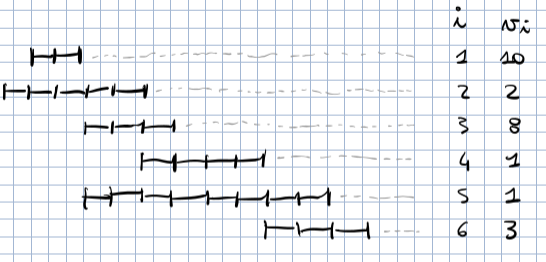
\includegraphics[scale = 0.7]{img/ta.png}
\end{center}
Per ogni attività si ha quindi un $s_i$, tempo di inizio, un $f_i$,
tempo di fine, e un $v_i$, il costo, con $i\ldots n$ che indica
l'attività. Definiamo $A\subseteq\{1,\ldots, n\}$ come l'insieme che
contiene attività mutualmente compatibili sse:
\[\forall i,j\in A\,\, [s_i,f_i)\cap [s_j,f_j)\neq \emptyset\]
definiamo anche $comp(A)$:
\[
  \begin{cases}
    $true$ & \mbox{ se mutualmente compatibili}\\
    $false$ & \mbox{ altrimenti}
  \end{cases}
\]
che verifica se dei task sono mutualmente compatibili.\\

Inoltre $V(A)=\sum_{i\in A}v_i$ per vedere il costo totale di una
serie di task, con:
\[P(\{1,\ldots, n\})\to \{true,\,false\}\]
\[V:P(\{1,\ldots, n\})\to \mathbb{R}\]
Quindi la soluzione sarà un insieme di task tale che:
\[S\subseteq \{1,\ldots, n\} \to
  comp(S)=true,\,\, V(S)=\max\{v(A)\}\]
Definiamo in maniera formale:
l'instanza è una $n\in\mathbb{N}$ e $X_n\in\{1,\ldots,n\}$. Ad ogni
attività $i\in X_n$ ci sono associate il tempo di inizio $s_i$, di fine $f_i$
e il valore $v_i$.\\
La soluzione è un sottoinsieme $S\subseteq X_N$ di attività
compatibili secondo la funzione \textit{comp} e tale che
$v(S)=\max_{A\subseteq X_n,\, comp(A)=TRUE}\{v(A)\}$.
La soluzione basata sulla forza bruta (calcolo tutte le combinazioni)
è $\Omega(2^n)$ nel caso migliore; non va bene.\\
Usiamo quindi la programmazione dinamica devo però prima cercare la
soluzione in termini ricorsivi, cercando i sottoproblemi. La struttura
da ``far calare'' è $X_n$ a step di $n-1$ lavorando quindi su
$S_{n-1}\subseteq X_{n-1}$ tale che valga quanto sopra.\\ Il
sottoprobelma i-esimo sarà $X_i=\{1,\ldots i\}$ con $S_i\subseteq X_i$
con le condizioni di sopra.\\
Il sottoproblema con $i=1$ avrà $X_1=\{1\}$ fatto solo dalla prima
attività e quindi avrò $S_1 = \{1\}$ e quindi $v(S_1)= v_1$, ovvero
$10$ nel nostro caso.\\
Inoltre se $i=0$ avrò l'insieme vuoto che ha valore 0. \\
Quindi $S_1 = \{1\}$, con $V(S_1)=1$, e $S_0 = \emptyset$, con
$v(s_0)=0$ e questi potrebbero essere i miei casi base. \\
Ragioniamo su 6, se 6 è soluzione allora sarà insieme alla soluzione
delle altre attività compatibili, ovvero quella di 4 essendo la prima
compatibile in ordine, o meglio $s_6 = \{6\}\cup S_4$. Per la 5 sarà
1, per la 4 sarà 2, per la 3 sarà 1 e per la 2 non sarà nessuna, come per
1, e quindi sarà 0. Ho appena definito $p(i) =\max\{j|\, j< i,\,
\mbox{ j compatibile con i}\}$ assumendo che $\max \emptyset = 0$,
quindi l'attività con indice maggiore compatibile precedente a quella
in studio.\\
\textbf{Questo schema funziona per attività ordinate sull'ordine di
  fine}.\\

Quindi:
\[
  S_i=\begin{cases}
    \{i\}\cup S_{p(i)} & \mbox{se }i\in S_i\\
    S_{i-1} & \mbox{se } i\not\in S_i
  \end{cases}
\]
e:
\[
  v(S_i)=\begin{cases}
    v_i+v(S_{p(i)})\\
    v(S_{i-1})
  \end{cases}
\]
Il modo di procedere consiste nel valcolare i valori e aggiornare il
massimo:
\[v(S_i)=\max\{v_i+v(S_{p(i)}),\, v(s_{i-1})\},\,i>0\]
sapendo $v(S_1)=1$ e $v(s_0) = 0$.\\
Ma in realtà $v(S_1)=1$ è ricavabile da $v(S_0)$ con la formula quindi
avremo solo un caso base: $v(S_0)=0,\,i=0$.\\
Quindi abbiamo trovato la ricorrenza, considerando anche che:
\[
  S_i=\begin{cases}
    \{i\}\cup S_{p(i)} & \mbox{se }v_i+v(S_{p(i)}) \geq v(S_{i-1})\\
    S_{i-1} & \mbox{se } v_i+v(S_{p(i)}) < v(S_{i-1}
  \end{cases}
\]
Quindi ottengo l'algoritmo ricorsivo per calcolare i vari $v_i$:
\begin{algorithm}
  \begin{algorithmic}
    \Function{$R\_OPT$}{$i$}
    \If{$i == 0$}
    \State \textbf{return} $0$
    \Else
    \State \textbf{return} $\max(v_i+R\_OPT(p[i]), R\_OPT(i-1))$
    \EndIf
    \EndFunction
  \end{algorithmic}  
\end{algorithm}
Ma è ingestibile dal punto di vista della complessità. Utilizzo quindi
un vettore $M[0..n]$, introducendo la programmazione dinamica,
dove in $M[i]$ memorizzo il valore della soluzione del problema di
taglia $i$, ovvero $v(S_i)$.\\
Facciamo quindi la ricorsione con l'annotazione:
\begin{algorithm}
  \begin{algorithmic}
    \For {$j\gets 0$ \textbf{to} $n$}
    \State $M[j]\gets \mbox{\textit{empty}}$
    \EndFor
    
    \Function{$AR\_OPT$}{$i$}
    \If{$M[i] == \mbox{\textit{empty}}$}
    \If {$i==0$}
    \State $M[i]\gets 0$
    \Else
    \State $M[i]\gets\max(v_i+AR\_OPT(p[i]), AR\_OPT(i-1))$
    \EndIf
    \EndIf
    \State \textbf{return} $M[i]$
    \EndFunction
  \end{algorithmic}  
\end{algorithm}
che resta una tecnica \textit{top-down}. Ma solitamente si lavora
\textit{bottom-up} nella programmazione dinamica. Quindi non abbiamo
di caricare l'array e non abbiamo bisogno di if/else:
\begin{algorithm}
  \begin{algorithmic}
    \Function{$PD\_OPT$}{$i$}
    \State $M[0]\gets 0$
    \For {$j\gets 1$ \textbf{to} $i$}
    \State $M[j]\gets\max(v_j+M[P[j]], M[J-1])$
    \EndFor
    \State \textbf{return} $M[i]$
    \EndFunction
  \end{algorithmic}  
\end{algorithm}
\textbf{ovviamente prima di tutto ho il caricamento di p[i], come è
  stato descritto sopra}.\\
Ora si ha una complessità pari a $\Theta(n)$ per quest'ultimo
algortimo, che calcola $v(S_i)$ ma bisogna sommare $\Theta(n\log n)$,
in quanto bisogna ordinare le attività sul tempo di fine.\\
Ora devo capire cos'è $S_i$, uso il \textbf{weighted interval
  scheduling} per stamparlo (usando l'array $M$), usando un algoritmo
ricorsivo che non ripete cose già usare, un algoritmo ricorsivo in
coda che quindi è comodo ed efficiente da lasciare ricorsivo:
\begin{algorithm}
  \begin{algorithmic}
    \Function{$WIS\_PRINT$}{$i$}
    \If {$i\neq 0$}
    \If {$v_i+M[p(i)] \geq M[i-1]$}
    \State $print(i)$
    \State $WIS\_PRINT(p(i))$
    \Else
    \State $WIS\_PRINT(i-1)$
    \EndIf
    \EndIf
    \EndFunction
  \end{algorithmic}  
\end{algorithm}
C'è uno step necessità di un teorema:
\begin{teorema}
  Siano $s_0,\ldots,S_{i-1}$ le varie soluzioni dei sottoproblemi allora:
  \[
    S_i=\begin{cases}
      \{i\}\cup S_{p(i)} & \mbox{se }i\in S_i\\
      S_{i-1} & \mbox{se } i\not\in S_i
    \end{cases}
  \]
\end{teorema}
\begin{proof}
  Assumo che $i\not\in S_i$. Se per assurdo $S_{i-1}\neq S_i$ e non
  fosse soluzione del problema i-esimo allora sicuramente
  $v(S_i)>v(S_{i-1})$. Siccome $i\not\in S_i$ allora
  $S_i\subseteq\{1,\ldots,i-1\}$ e quindi $comp(S_i)=TRUE$ ma questo
  comporta un assurdo, infatti so che $S_{i-1}$ è soluzione di $i-1$
  ma lo sarebbe anche $S_i$ ma so che $v(S_i)>v(S_{i-1})$ quindi
  $S_{i-1}$ non sarebbe soluzione di $i-1$; quindi abbiamo un assurdo
  dato da una contraddizione.
  \textbf{resto della dimostrazione settimana prossima}
\end{proof}
\subsection{Basi di Programmazione Dinamica}
Un problema di decisione prevede unicamente 2 tipi di risultato: vero
e falso. Si ha una distinzione dei problemi:
\begin{itemize}
  \item \textbf{problemi intrattabili}, che potrebbero avere una
  risposta calcolabile in un tempo idnefinito o addirrittura che non
  possono essere dimostrati
  \item \textbf{problemi di ricerca}, che si occupano di trovare una
  soluzione positiva ad una certa istanza (per esempio dei problemi
  che trattano i percorsi)
  \item \textbf{problemi di ottimo}, dove si cerca una e una sola
  soluzione che massimizza o minimizza una certa funzione costo
\end{itemize}
Si parla di \textbf{algoritmi euristici} quando si una un algoritmo
che ci da una soluzione che magari non è la migliore. A questi si
aggiungono \textbf{algortitmi di approssimazione} che si occupano di
cercare l'ordine di una soluzione rispetto a quella ``migliore''.
\subsection{Un Problema di Sequenze}
Prendiamo una stringa $X=<x_1,\ldots,x_n>$. Una sottosequenza di $X$ è
un insieme di indici con $i_1\ldots i_k$ con $k\leq n$ e indici
strettamente crescenti ma non necessariamente consecutivi. Quindi data
una sequenza $X=<x_1,\ldots,x_n>$ e una sottosequenza $Z=<z_1,\ldots
z_n>$ diciamo che:
\[\exists i_1,\ldots i_k \to x_{i_1}< x_{i_2} < \cdots < x_{i_k},\,\,
  i_i > i_{i-1}\]
\textit{Si assuma che gli indici partano da 1}.\\
Quindi, per esempio, per la stringa $X=<A,B,C,B,D,A,B>$ si possono
avere le sottosequenze $A_1 = <B,C,D,B>$ (con indici $2,3,5,7$),
$A_2=<A,B,A,B>$ (con indici $1,2,6,7$ oppure $1,4,6,7$) etc$\ldots$.
\subsection{Longest Common Substring}
Si definisce una \textbf{sottosequenza comune} $Z$ a due sequenze $X$ e
$Y$ se $Z$ è sottosequenza sia di $X$ che di $Y$ (non è necessario che
gli indici siano nello stesso ordine).\\
Cerchiamo ora un algoritmo che trovi la più grande sottostringa
comune, appunto \textbf{long common substring
  (LCS)}, con però elementi ordinati in grandezza, quindi
\textit{longest increasing subsequence (LIS)}.\\
Con una soluzione iterativa avremmo $O(2^n)$ quindi pensiamo
ad una soluzione con la programmazione dinamica.\\
Cerchiamo quindi un problema associato, cercando la sottoesequenza di
$X$ più lunga che termina in una certa posizione $i$. In questo studio
delle sequenze gli indici aumentano solo se il valore che indicizzano
è superiore a quello rpecedente, altrimenti diminuisocno di una unità
(a meno che non sia l'indice 1 che resta uguale),
quindi, per esempio, la stringa $X=<A,B,C,B,D,A,B>$ avrà indici
$1,2,3,2,4,3,4$.\\
Definiamo $L[i]$ la lunghezza massim della LIS che termina col
carattere in posizione $i$.\\
Procedo salvando la lunghezza della sottosequenza iù lunga fino a
$i$.\\
Si definisce $X_i$ la restrizione della sequenza considerando
solo i primi $i$ caratteri. Chiamiamo $Z_i$ la più lunga sottosequenza
di $X$ che termina con $X_i$. Salviamo le varie $Z$ in un array
$L[1..N]$ con $L[i]$ che è la lunghezza massima della sottosequenza
di $X$ che termina con $X_i$
\\
Si ha il caso base:
\[L[1]=1\]
e il caso generale:
\[L[i]=1+\max_{1\leq j\leq i-1} \{L[j]|\,X_j<X_i\},\,\, 1 <i\leq N\]
ricordando che $\max{\emptyset}=0$.\\
La soluzione sarà quindi:
\[\max_{1\leq i \leq N}\{L[i]\}\]
Scriviamo quindi l'algoritmo:
\begin{algorithm}
  \begin{algorithmic}
    \Function {$LIS$}{$X[1..N]$}
    \State $L[1..N]$
    \State $X[0]=-1$
    \State $L[1]=1$
    \State $L[0]=0$
    \For {$i\gets 2$ \textbf{to} $N$}
    \State $R\gets maxAcc(l[], i, i-1, X[i])$
    \State $L[i]=R+1$
    \EndFor
    \State $RT\gets \max(L[i],1,N)$
    \State \Return $RT$
    \EndFunction
  \end{algorithmic}
\end{algorithm}
Con la funzione \textit{maxAcc} che calcola il massimo degli
accettabili. Questo algoritmo è $O(n^2)$.\\
calcolo $L[i]$ che è la sequenza più lunga che termina col carattere i:
\[
  L[i]=]\begin{cases}
    0 & i=0\\
    1 & i=1\\
    1+\max(L[j]|\, c[j]<c[i],\, j=1\ldots i-1)  & i>1 
  \end{cases}
\]
Scriviamo il vero algoritmo:
\begin{algorithm}
  \begin{algorithmic}
    \Function{$LIS$}{$S[1..n]$}
    \State $L[1]\gets1$
    \State $maxTot \gets 1$
    \For {$i\gets 2$ \textbf{to} $n$}
    \State $max \gets 0$
    \For {$j\gets 1$ \textbf{to} $i-1$}
    \If{$S[j] < S[i]$ \textbf{AND} $L[i]>max$}
    \State $max \gets j$
    \EndIf
    \State $l[i]\gets L[max]+1$
    \State $P[i]\gets max$ 
    \If {$L[i]> maxTot$}
    \State $maxTot \gets i$
    \EndIf
    \EndFor
    \EndFor
    \State \textbf{return} $maxTot$
    \EndFunction
  \end{algorithmic}
\end{algorithm}
Con \textit{maxTot} salva il massimo dell'arrayb delle lunghezza.\\
Che ha tempo di esecuzione pari a $T(n)=3c+5cn+3c\sum_1^ni=O(n^2)$.\\
Questa funzione verrà chiamata in una ciclo $for$. Per rendere il
tutto più efficiente quindi memorizzo, anzichè memorizzare tutti i
valori degli array che si vengono a creare contenenti le sequenze
buone, l'indice del maxTot precedente, nella lista $P$, avendo una
complessità di salvataggio sulla memoria pari a $O(n)$.\\
\subsection{Il Problema delle Scatole}
Ho una tripla $B_i=(a_i,b_i,c_i)$ rappresentanti lunghezza, larghezza
e altezza di una scatola. $B_i$ è quindi un insieme di scatole che non
possono essere ruotate. Voglio sapere a lunghezza più lunga di scatole
che possono essere contenute una dentro l’altra. Cerco quindi il
massimo valore di $k$ tale per cui, per una sequenza $ B_1,\ldots,B_i$:
\[\exists x\to B_1,\ldots,B_i|\,B_{i1}\subset B_{i2}\subset\cdots
  \subset B_{ik},\,\,i_1<\cdots<i_k\]
Si introduce un vettore $z$ con $n$ elementi tale che $z[i]$ sia la
lunghezza massima di una sottosequenza crescente di elementi $
B_1,\ldots,B_i$. Quindi:
\[
  z[i]=\begin{cases}
    1+\max\{z[j]|\, 1\leq j < i,\,a_j<a_i,\,b_j<b_i,\,c_j<c_i\} &
    i>1\\
    1 & i = 1
  \end{cases}
\]
inoltre $\max\{\emptyset\}=0$. Abbiamo quindi il seguente algoritmo:

\begin{algorithm}
  \begin{algorithmic}
    \Function {MaxBox}{B[1..n]}
    \State $z[1]\gets 1$
    \For{$i\gets 2$ \textbf{to} $n$}
    \State $max \gets 0$
    \For{$j\gets 1$ \textbf{to} $i-1$}
    \If {$a_j<a_i$ \textbf{AND} $b_j<b_i$ \textbf{AND} $c_j<c_i$ \textbf{AND} $z[j]<max$ }
    \State $max\gets z[j]$
    \EndIf
    \EndFor
    \State $z[i]\gets max$
    \EndFor
    \State \textbf{return} $z$ 
    \EndFunction
  \end{algorithmic}
\end{algorithm}


Si ha complessità apri a $O(n^2)$ mentre lo spazio richiesto è quello
per memorizzare il vettore, ovvero $\Theta(n)$.\\
Può anche essere scritto ricorsivamente ma risulta troppo esoso in
termini di spazio.
\section{Longest Common Subsequence}
Ritorniamo al problema di inizio capitolo. Abbiamo due stringhe,
$X=<x_1,\ldots x_n>$ e $Y=<y_1\ldots y_n>$ con $Z$ sottosequenza
comune a $X$ e $Y$.\\
Per ragionare secondo la programmazione dinamica identifichiamo le
istanze relative ai sottoproblemi come $X_i$ e $Y_j$ che sono $n+1$ e
$m+1$ prefissi del problema. Un sottoproblema generico è identificato
da una coppia di indici e ad ogni sottoproblema è associata una
lunghezza. L alunghezza della massima sottosequenza comune $K$ è la
maggiore tra tutte le lunghezze delle sottosequenze comuni $W$.
Si ha quindi che:
\[Z_k=LCS(X_i, Y_j)\]
Inoltre si ha che, sapendo che $x_i$ è l'ultimo simbolo:
\[LCS(x_{i-1},y_{j-1})\, |\, x_i  \mbox{ se } x_i=y_j\]
altrimenti, se $z_k\neq x$, si ha che:
\[Z_{k}=LCS\left(X_{i}, Y_{j}\right)=LCS\left(X_{i-1},
    Y_{j}\right)   \text { e } C_{i, j}=C_{i-1, j}\]
mentre, se $x_x\neq y_j$ si ha che:
\[Z_k=LCS\left(X_{i}, Y_{j}\right)=LCS\left(X_{i}, Y_{j-1}\right)
  \text { e } C_{i, j}=C_{i, j-1}\]
Quindi cerco un algoritmo del tipo:
\[LCS(x,y)\to LCS(x-\{A\},y-\{A\})\]
Costruisco quindi una matrice $C$ che indica come sono allineate le
sequenze con un algoritmo che controlla i primi $i$ caratteri di
$X$ e i primi $j$ di $Y$.

La prima riga e la prima colonna sono fissi 0, e il controllo inizia
dalla prima riga di 0. Non appena l’algoritmo trova un match, copia
nella casella della matrice corrispondente il valore contenuto nella
casella precedente sulla diagonale a sinistra, incrementandolo di 1,
mentre se i caratteri confrontati sono diversi viene copiato nella
casella il massimo tra il valore a sinistra e il calore
sopra. L'ultima casella in basso a destra (quella di posizione
$(n,m)$) rappresenta la lunghezza massima.\\
Quindi $C[i,j]$ contiene la lunghezza della stringa più lunga tra gli
$i$ caratteri di $X$ e i $j$ di $Y$.\\
Si ha quindi un caso base sfruttando la prima riga e la prima colonna
formate da soli zeri:
\[C[i,j]=0 \mbox{ se } i=j=0\]
e un caos generico:
\[C[i,j]=
  \begin{cases}
    C[i-1, j-1]+1 & \mbox{se } x_i=y_i\\
    \max \{C[i-1, j], C[i, j-1]\} & \mbox{se } x_i\neq y_i
  \end{cases}
\]
per esempio per $X=<A,B,C,B,D,A,B>$ e $Y=<B,D,C,A,B,A>$ avremmo:
\begin{center}
  \begin{tabular}{|c|c|c|c|c|c|c|c|}
    \hline
    X / Y & {0} & {B} & {D} & {C} & {A} & {B} & {A} \\
    \hline
    0 & {0} & {0} & {0} & {0} & {0} & {0} & {0} \\
    \hline
    A & {0} & {0} & {0} & {0} & {1} & {1} & {1} \\
    \hline
    B & {0} & {1} & {1} & {1} & {1} & {2} & {2} \\
    \hline
    C & {0} & {1} & {1} & {2} & {2} & {2} & {2} \\
    \hline
    B & {0} & {1} & {1} & {2} & {2} & {3} & {3} \\
    \hline
    D & {0} & {1} & {2} & {2} & {2} & {3} & {3} \\
    \hline
    A & {0} & {1} & {2} & {2} & {3} & {3} & {4} \\
    \hline
    B & {0} & {1} & {2} & {2} & {3} & {4} & {4} \\
    \hline
  \end{tabular}
\end{center}

ottengo quindi:
\begin{algorithm}[H]
  \begin{algorithmic}
    \Function{$LCS$}{$X,Y$}
    \For {$i\gets 0$ \textbf{to} $n$}
    \State $C[i,0]\gets 0$
    \EndFor
    \For {$j\gets 0$ \textbf{to} $m$}
    \State $C[0,j]\gets 0$
    \EndFor
    \For {$1\gets 1$ \textbf{to} $n$}
    \For {$j\gets 1$ \textbf{to} $m$}
    \If {$X[i]==Y[j]$}
    \State $C[i,j]\gets C[i-1,j-1]+1$
    \Else
    \State $C[i, j]\gets\max(C[i-1, j], C[i, j-1])$
    \EndIf
    \EndFor
    \EndFor
    \State \textbf{return} $C[n,m]$
    \EndFunction
  \end{algorithmic}
\end{algorithm}
Ho quindi un tempo $\Theta(nm)\sim \Theta(n^2)$ e uno spazio richiesto
pari a $\theta(nm)$ che è quello della matrice.\\
La sottosequenza poi la prendo usando gli indici $i$ e $j$\\
Per risparmiare spazio posso riempire la matrice cancellando le righe
inutili, quindi al peggio uso due righe, quella he sto costruendo e
quella precedente, raggiungendo $\Theta(2n)$ come uso di spazio ma
rendendo più difficile la risalita per ritrovare quale è
effettivamente la sequenza, in quanto dovrei risalire la matrice
costruendola nuovamente.\\
L'algoritmo di riscostruzione della stringa è il seguente, prendendo
in ingresso le due stringhe e la matrice appena caricata:
\begin{algorithm}[H]
  \begin{algorithmic}
    \Function {$buildLCS$}{$X,Y,C$}
    \State $result \gets null$
    \State $i\gets length(X)$
    \State $j\gets length(Y)$
    \While {$i>0$\textbf{ AND }$j>0$}
    \If {$X[i]==Y[j]$}
    \State $result\gets X[i]+result$
    \State $i\gets i-1$
    \State $j\gets j-1$
    \Else
    \If {$C[i-1,j]>C[i,j-1]$}
    \State $i\gets i-1$
    \Else
    \State $j\gets j-1$
    \EndIf
    \EndIf
    \EndWhile
    \State \textbf{return }$result$
    \EndFunction
  \end{algorithmic}
\end{algorithm}
Quindi parto dall'ultima casella in basso a destra, se corrisponde a
due caratteri uguali salvo il carattere e mi sposto indietro sulla
diagonale. Altrimenti vedo se il valore sopra è maggiore di quello
a sinistra e in quel caso mi sposto su quello, altrimenti mi sposto su
quello a sinistra e ricomincio da 0 finchè non arrivo a fine
matrice.\\
Trovo così una sottostringa in quanto se la casella a sinistra è
uguale a quella sopra devo prendere entrambe le direzioni, geneando
così $K$ LCS tutte corrette.
\subsection{Growing LCS, GLCS}
Cerco una LCS in cui gli elementi sono oridnati in ordine crescente.
Suppngo di avere $X=[1,4,12,3,16,8]$ e $Y=[12,1,3,17,8]$. La $Z$
sarebbe quindi $Z=[1,3,8]$.\\
Una soluzione banale è trovare tutte le sottosequenze, calcolando la
lunghezza solo di quelle crescenti, ma avrebbe tempo esponenziale.\\
Sfruttando la programmazione dinamica controllo ogni volta che la
sottosequenza comune precedente sia comparibile (che quindi sia
crescente) aggiungendo anche un ulteriore carattere. Sfrutto la stessa
logica della LCS con la matrice $C[n,m]$ con $n$ lunghezza di $X$ e
$m$ lunghezza di $Y$. Identifichiamo con $C[i,j]$ il numero di
caratteri che compongono la più lunga sottosequenza comune crescente
che termina con $x_i=y_i$.\\
Si ottiene la seguente equazione di ricorrenza:
\[
  \begin{cases}
    G[i,j] = 0 & \mbox{ se } x_i\neq y_i\\
    G[i,j] = \max\{C[a,b]|\, 1\leq a\leq i,\,1\leq b \leq m,\, x_a<
    x_i,\, y_b< y_j\}+1 & \mbox{ se } x_i=y_j\}
  \end{cases}
\]
Come per LCS le caselle corrispondenti a caratteri che non matchano
vengono settate a 0. Quando invece si ha un match tra i due caratteri
si inserisce il valore della più lunga sottosequenza comune
precedente, che viene ricercata tra tutti i valori precedenti, 
aggiungendo 1. Alla fine della compilazione della tabella si cerca il
massimo tra tutte le caselle. Nel complesso si hanno 4 cicli per la
costruzione più altri 2 cicli per la ricerca del massimo. Nel
complesso si ottiene $\Theta(n^2m^2)\sum \Theta(n^4)$ con unon spazio
pari $\Theta(nm)$.\\
Prendendo $X=<1,4,12,3,7,16,8,1>$ e $y=<12,1,3,17,8,1>$
oettengo:
\begin{center}
  \begin{tabular}{|c|c|c|c|c|c|c|c|c|}
    \hline
    $X/Y$ & {1} & {4} & {12} & {3} & {7} & {16} & {8} & {1}\\
    \hline
    {12} & {0} & {0} & {1} & {0} & {0} & {0} & {0} & {0}\\
    \hline
    {1} & {1} & {0} & {0} & {0} & {0} & {0} & {0} & {1}\\
    \hline
    {3} & {0} & {0} & {0} & {2} & {0} & {0} & {0} & {0} \\
    \hline
    {17} & {0} & {0} & {0} & {0} & {0} & {0} & {0} & {0}\\
    \hline
    {8} & {0} & {0} & {0} & {0} & {0} & {0} & {3} & {0}\\
    \hline
    {1} & {1} & {0} & {0} & {0} & {0} & {0} & {0} & {1}\\
    \hline
  \end{tabular}
\end{center}
Quindi il massimo è 3.\\
vediamo qundi l'algoritmo:
\begin{algorithm}[H]
  \begin{algorithmic}
    \Function {$GLCS$}{$X,Y$}
    \For {$i\gets 1$ \textbf{to} $n$}
    \For {$j\gets 1$ \textbf{to} $m$}
    \If {$X[i]\neq Y[j]$}
    \State $G[i,j]\gets 0$
    \Else
    \State $max\gets 0$
    \For {$a\gets 1$ \textbf{to} $i-1$}
    \For {$b\gets 1$ \textbf{to} $j-1$}
    \If {$G[a,b] > max$ \textbf{AND} $x[a]<x[i]$}
    \State $max \gets G[a,b]$
    \EndIf
    \EndFor
    \EndFor
    \State $g[i,j] \gets max +1$
    \EndIf
    \EndFor
    \EndFor
    \State $maxtot \gets 0$
    \For {$i\gets 1$ \textbf{to} $n$}
    \For {$j\gets 1$ \textbf{to} $m$}
    \If {$G[i,j]>maxtot$}
    \State $maxtot \gets G[i,j]$
    \EndIf
    \EndFor
    \EndFor
    \State \textbf{return} $maxtot$
    \EndFunction
  \end{algorithmic}
\end{algorithm}
\newpage
\subsection{Heaviest Common Subsequence (HCS)}
Vediamo un'altra variante della LCS, dove ogni elemento delle stringhe
$X$ e $Y$ viene associato ad un peso e si cerca la sequenza comune più
pesante (che non è necessariamente la più lunga). Analizziamo le
stringhe $X=<A,B,C,B,A,D,E>$ e $Y=<D,A,B,B,A,E>$ dove si hanno i
seguenti pesi:
\[pesi=
  \begin{cases}
    W(A)=1\\
    W(B)=1\\
    W(C)=2\\
    W(D)=30\\
    W(E)=20
  \end{cases}
\]
L'algoritmo è simile a quello di LCS ma ad ogni aggiornamento della
sequenza comune va aggiunto il peso del nuovo elemento.\\
Definiamo $P[i,j]$ il peso massimo della sottosequenza comune a $X$ e
$Y$ ristretta ai primi $i$ caratteri di $X$ e ai primi $j$ di $Y$.\\
Si ottiene quindi:
\[
  P[i,j]=\begin{cases}
    P[i-1,j-1]+w(X[i]) & \mbox{ se } x_i=y_i\\
    \max\{P[i-1,j],P[i, j-1]\} & \mbox{ se } x_i=y_i
  \end{cases}
\]
inoltre $P[i,j]=0$ se entrambi gli indici sono nulli.
Come per LCS la soluzione si troverà nell'ultima posizione a destra
della matrice, ovvero in $P[n,m]$. Per le stringhe si otterrebbe una
matrice così:
\begin{center}
  \begin{tabular}{|c|c|c|c|c|c|c|c|c|}
    \hline
    X / Y & {0} & {A} & {B} & {C} & {B} & {A} & {D} & {E} \\
    \hline
    {0} & {0} & {0} & {0} & {0} & {0} & {0} & {0} & {0} \\
    \hline
    {D} & {0} & {0} & {0} & {0} & {0} & {0} & {30} & {30} \\
    \hline
    {A} & {0} & {1} & {1} & {1} & {1} & {1} & {30} & {30}\\
    \hline
    {B} & {0} & {1} & {2} & {2} & {2} & {2} & {30} & {30}\\
    \hline
    {B} & {0} & {1} & {1} & {2} & {5} & {3} & {30} & {30}\\
    \hline
    {A} & {0} & {1} & {2} & {2} & {3} & {4} & {30} & {30}\\
    \hline
    {E} & {0} & {1} & {2} & {2} & {3} & {4} & {30} & {50}\\
    \hline
  \end{tabular}
\end{center}
\textit{Per ricostruire la sequenza, partiamo dall’ultima casella in
  basso a destra e controllo se ho migliorato in diagonale (in tal
  caso quello è un elemento della sottosequenza comune). Altrimenti
  vado a vedere dove ho preso il massimo in verticale o orizzontale,
  naturalmente non considerando tali caratteri come appartenenti alla
  sottosequenza.}
\newpage
Vediamo l'algoritmo:
\begin{algorithm}
  \begin{algorithmic}
    \Function {$HCS$}{$X,Y$}
    \For {$i\gets 0$ \textbf{to} $n$}
    \State $C[i,0]\gets 0$
    \EndFor
    \For {$j\gets 0$ \textbf{to} $m$}
    \State $C[0,j]\gets 0$
    \EndFor
    \For {$i\gets 1$ \textbf{to} $n$}
    \For {$j\gets 1$ \textbf{to} $m$}
    \If {$X[i]==Y[j]$}
    \State $C[i,j]\gets C[i-1,j-1]+w(X[i])$
    \Else
    \State $C[i,j]\gets C[i-1,j]$
    \If {$C[i,j-1] > C[i-1,j]$}
    \State $C[i,j]\gets C[i, j-1]$
    \EndIf
    \EndIf
    \EndFor
    \EndFor
    \State \textbf{return} $C[n,m]$
    \EndFunction
  \end{algorithmic}
\end{algorithm}
L'algortimo richiede $\Theta(nm)$ sia come tempo che come spazio
\subsection{ALCS}
Parliamo di \textit{Alternanting LCS}. Ipotizziamo sequenze
numeriche. Cerchiamo la più lunga sottosequenze comune che rispetti
una certa alternanza. Per esempio analizziamo il pari e dispari.
Parto da LCS e vedo come modificarlo. Creo una matrice $M[i,j]$ che
contiene le lunghezze delle LCS alternante considerando i primi $i$
caratteri della prima sequenza $X$ e i primi $j$ di $Y$.\\
Si ha quindi innazitutto che:
\[ M[i,j]=
  \begin{cases}
    \max\{M[i-1,j], M[i,j-1]\} & \mbox{ se } X_i\neq Y_j\\
    1+M[i-1,j-1] & \mbox{ se } X_i=Y_j
  \end{cases}
\]
ma non si ha rappresentazione dell'alternanza pari/dispari, diventa
quindi cge $M[i,j]$ conterrà la LCS alternante che termina con  $X_i$
e $Y_j$. Diventa quindi:
\[ M[i,j]=
  \begin{cases}
    0 & \mbox{ se } X_i\neq Y_j\\
    1+\max\{M[a,b]|\, 1\leq a \leq i,\,\,1\leq b\leq j,\,\,and\,\,
    (x_a\,mod\, 2 \neq x_b\,mod\, 2)\} & \mbox{ se } X_i=Y_j
  \end{cases}
\]
La soluzione quindi è il valore più grande contenuto nella matrice:
\[L=\max\{M[i,j]|\,1\leq i\leq n,\, 1\leq j\leq m\}\]
L'algoritmo deriva direttamente dall'equazione di ricorrenza\\
Per riempire ho tempo $\Theta(n^4)$ e spazio $\Theta(n^2)$
\section{Problemi di Ottimo}
\subsection{Problema Knapsack (dello zaino)}
Sia data una serie di oggetti appartentenenti all'insieme
$X_n=\{1,\ldots, n\}$. $\forall i \in X_n$ si hanno due variabili:
$v_i$ corrispondente al valore di un oggetto e $w_i$ corrispondente al
peso di quell'oggetto. Il problema da risolvere consiste nel riempire
uno zaino di capacità $L$ con la combinazione ottimale di oggetti che
massimizzi il valore. Voglio quindi una soluzione $S_n\subseteq X_n$.
Avendo in ballo peso e valore useremo una matrice $M[n,L]$, dove
$M[i,j]$ rappresenterà il massimo valore ottenibile scegliendo tra i
primi $i$ oggetti per avere peso $S$. Formalmente si avrà:
\[
  \begin{cases}
    M[0,j]=0\\
    M[i,0]=0\\
    M[i,j]=\max\{M[i-1,j], M[i-1, j-w_i]+v_i\}
  \end{cases}
\]
E la soluzione sarà il valore contenuto nell'ultima casella
$M[n,L]$.\\
Vediamo un esempio di matrice, con $X=\{1,2,3,4,5\}$, $V=\{1,6,18,22,28\}$,
$W=\{1,2,5,6,7\}$ e $L=11$:
\begin{center}
  \begin{tabular}{c|cccccccccccc}
    $X/L$ & 0 & 1 & 2 & 3 & 4 & 5 & 6 & 7 & 8 & 9 & 10 & 11\\
    \hline
    0 & 0 & 0 & 0 & 0 & 0 & 0 & 0 & 0 & 0 & 0 & 0 & 0\\
    1 & 0 & 1 & 0 & 0 & 0 & 0 & 0 & 0 & 0 & 0 & 0 & 0\\
    2 & 0 & 1 & 6 & 7 & 0 & 0 & 0 & 0 & 0 & 0 & 0 & 0\\
    3 & 0 & 1 & 6 & 7 & 0 & 18 & 19 & 24 & 25 & 0 & 0 & 0\\
    4 & 0 & 1 & 6 & 7 & 0 & 18 & 22 & 24 & 29 & 29 & 0 & 0\\
    5 & 0 & 1 & 6 & 7 & 0 & 18 & 22 & 28 & 29 & 34 & 35 & 40\\
  \end{tabular}
\end{center}
Dove la soluzione è appunto 40.\\
Questo algoritmo lavora in tempo $\Theta(nL)$ e in spazio
$\Theta(nL)\sim \Theta(L))$. Questo algoritmo funziona su $L$
comparabile al numero dei pesi nonostante sia
\textit{NP-complete}, con tempo esponenziale e di difficile
risoluzione negli altri casi.

\newpage
Vediamo ora l'algoritmo ($n$ è il numero di oggetti):
\begin{algorithm}[H]
  \begin{algorithmic}
    \Function{$Knapsack$}{$X,v,w,L$}
    \For{$j\gets 1$\textbf{ to }$L$}
    \State $M[0,j]\gets 0$
    \EndFor
    \For{$i\gets 1$\textbf{ to }$n$}
    \State $M[i,0]\gets 0$
    \EndFor
    \For{$i\gets 2$\textbf{ to }$n$}
    \For{$j\gets 2$\textbf{ to }$L$}
    \If{$w_i>j$}
    \State $M[i,j]\gets M[i-1,j]$
    \Else
    \State $M[i,j]\gets \max\{M[i-1,j],M[i-1,j-w_i]+v_i\}$
    \EndIf
    \EndFor
    \EndFor
    \State \textbf{return} $M[n,L]$
    \EndFunction
  \end{algorithmic}
\end{algorithm}
\chapter{Programmazione Greedy}
\section{Subset Sum}
Sia dato un insieme di oggetti $X_n=\{1,\ldots, n\}$, ognuno con un
certo valore $v_i$. Si ricerca un sottoinsieme che come somma dei
valori un certo valore $k$. Siamo di fronte ad un altro problema
\textit{pseudo-polinomiale} (è polinomiale se $k\sim n$).\\
Come appoggio usiamo una matrice $M[n+1,k]$ di booleani tale che:
\[M[i,j]=
  \begin{cases}
    T & \mbox{ se esiste un sottoinsieme dei primi i elementi di
      valore totale j}\\
    F & \mbox{ altrimenti}
  \end{cases}
\]
quindi, dopo aver posto $0$ ovunque si ha $i=0$ (la prima colonna), si
ha:
\[M[i,j]=
  \begin{cases}
    T & \mbox{ se } v_i=j\\
    M[i-1,j]\,\,OR\,\, M[i-1,j-v_i] & \mbox{ se } j-v_i>0
  \end{cases}
\]
Cerchiamo ora la soluzione. Se $M[n,k]=0$ allora non esiste nessun
sottoinsieme di valore $k$. Invece se $M[n,k]=1$ bisogna risalire la
matrice per trovare gli elementi appartenetenti alla soluzione.\\
\newpage
Quindi si avrà:
\begin{algorithm}[H]
  \begin{algorithmic}
    \Function {$SubsetSum$}{$X,n,k$}
    \State $posR\gets n$
    \State $posC\gets k$
    \While {$posC>0$}
    \If {$M[posR-1][posC] == T$}
    \State $print(posR)$
    \State $posC\gets posC - v[posR]$
    \EndIf
    \State $posr \gets posR-1$
    \EndWhile
    \EndFunction
  \end{algorithmic}
\end{algorithm}
\section{Knapsack frazionario}
Vediamo ora un esempio di \textbf{programmazione greedy}, ricordando
che questa tecnica:
\begin{algorithm}
  \textit{riguarda problemi che hanno l’obiettivo di arrivare al
    risultato ottimo utilizzando sottostrutture ottime locali.}
\end{algorithm}
Vediamo ora \textit{knapsack frazionario} che, a differenza
dell'algoritmo orginale, prevede che un oggetto possa essere preso
anche parzialmente. Si indica con $w_i$ il peso degli oggetti e con
$v_i$ il loro valore. Chiamiamo $L$ la capacità dello zaino e con
$p_i$ il profitto di un oggetto:
\[p_i=\frac{v_i}{w_i}\]
Cerco quindi di massimizzare il profitto.\\
Procedo quindi ordinando, usando quindi la tecncia greedy, gli oggetti
in ordine decrescente rispetto al profitto e inserendo gli oggetti
sfruttando questo ordine fin tanto che il peso dell'oggetto che sto
inserendo non è maggiore alla capacità residua. A questo punto
frazioniamo l'oggetto (che prende il nome di \textbf{oggetto
  critico}). Si ha quindi il caso migliore nel caso non si debba mai
frazionare e si ha tempo $O(n\log n)$ (usando, per esempio, mergesort)
per l'ordinamento e $O(n)$ per la scelta.
\newpage
Si ha quindi (con $P$
vettore dei profitti, $W$ vettore dei pesi, $V$ vettore dei valori,
$n$ numero degli oggetti e $L$ peso massimo trasportabile):
\begin{algorithm}[H]
  \begin{algorithmic}
    \Function {$Knap\_frazionario$} {$V,W,n,L$}
    \State $s\gets 0$
    \State $peso\gets 0$
    \For{$i\gets 1$ \textbf{to} $n$}
    \State
    \State $R[i]\gets \frac{V[i]}{W[i]}$
    \EndFor
    \State $mergesort(R)$
    \State $i\gets 1$
    \While{$peso<L$ \textbf{AND} $i\leq n$}
    \If{$W[i]+peso\leq L$}
    \State $s\gets s+1$
    \Else
    \State $s\gets s+\frac{(L-p)}{W[i]}$
    \EndIf
    \State $peso\gets peso+W[i]$
    \State $i\gets i+1$
    \EndWhile
    \State \textbf{return} $s$
    \EndFunction
  \end{algorithmic}
\end{algorithm}
Si ha quindi $O(n\log n)$ e dipende solo dal numero di oggetti, si ha
quindi un algortimo polinomiale.
\section{Approfondimento Greedy}
Come abbiamo visto con knapsack frazionario facciamo una scelta
\textit{greedy} nel momento in cui prendo la spluzione che mi sembra
migliore in un dato momento, infatti queste scelte sono dette
\textit{localmente ottime}.\\
\textbf{I problemi di ottimo in cui si riesce ad arrivare ad una soluzione di
  ottimo mediante una sequenza di soluzioni localmente ottima
  ammettono smepre una soluzione greedy}.\\
Un algoritmo greedy segue un certo schema. Parto inizializzando un insieme
di soluzioni a vuoto, eventualmente calcolo il parametro di selezione,
ordino gli elementi in base a quel parametro e infine per ogni
elemento vedo se appartiene alle soluzioni. In questo modo si impiega
$O(n\log n)$ per ordinare e $O(n)$ per scegliere.\\
\section{Problema dell'Autostrada}
Si ipotizzi di essere all'inizio di un'autostrada (al kilometro 0) di
lunghezza $N$. Si ipotizzi di avere $R$ kilometri di autonomia e che
ci siano $n$ pompe di benzina. Si cerca di minimizzare il numero di
soste.\\
Usiamo la tecnica greedy e ordiniamo il vettore delle soste, sapendo
che ci fermeremo sse la stazione successiva è fuori portata. Vediamo
quindi l'algortimo, sapendo che $K$ è il vettore delle soste, $S$
vettore delle soluzioni (si usa notazione insiemistica nello psuedo
codice) e $R$ è l'autonomia in kilometri:
\begin{algorithm}[H]
  \begin{algorithmic}
    \Function {$Sosta$}{$K, R$}
    \State $S\gets \emptyset$
    \State $pos\gets 0$
    \State $mergesort(K)$
    \For{$i\gets 1$ \textbf{to} $n-1$}
    \If{$K[i]\geq pos + R$ \textbf{AND} $K[i+1]>pos+R$}
    \State $S\gets S\cup K[i]$
    \State $pos \gets K[i]$
    \EndIf
    \EndFor
    \If{$K[i]\geq pos + R$ \textbf{AND} $N>pos+R$}
    \State $S\gets S\cup K[N]$
    \State $pos \gets K[N]$
    \EndIf
    \State \textbf{return }$S$
    \EndFunction
  \end{algorithmic}
\end{algorithm}
Ma non stiamo analizzando il caso in cui due stazioni distino più di
$R$, ma questo a livello teoirco lo possiamo ovviare dando per
scontato ipotizzando che l'input sia corretto (ovvero che $K$ non
permetta questa situazione). Come Dimostrato sopra si ha $O(n\log n$)
\section{TSP}
Vediamo il problema del \textit{traveling saleman problem (TSP)}. Si
ha che un viaggiatore deve visitare una e una sola volta tutte le $N$
città in cui deve vendere i prodotti. Vuole minimizzare il costo per
fare il giro completo delle città e tornare al punto di partenza. Si
ha che ogni città è collegata ad ogni altra con un certo peso (che
rappresenta il costo che si deve pagare per spostarsi tra le due
città).\\
Una possibile soluzione greedy consiste nel scegliere sempre il
cammino meno ``pesante'', ma questo rischia di far perdere alcune
combinazioni di cammini che insieme ``costerebbero'' meno, perdendo
quindi la soluzione migliore. Possiamo concludere che non si può
risolvere con la programmazione greedy in maniera ottimizzata.
\section{Matroidi}
Con il problema del TSP abbiamo visto che non sempre si può arrivare
ad una soluzione con la programmazione greedy. Cerchiamo quindi uno
strumento teorico per stabilire a priori se si può arrivare ad una
soluzione con la programmazione greedy. Questo strumento è detto
\textbf{matroide}.
\begin{definizione}
  Si definisce un \textbf{sistema di indipendenza} $<E,F>$. Si ha che
  $F$ è l'insieme di tutti i possibili sottoinsiemi construibili a
  partire dagli elementi di $E$, che è un insieme finito. $F$ è quindi
  \textbf{l'insieme delle parti} di $E$. La coppia $<E,F>$ è sistema
  di indipendenza sse:
  \[\forall A\in F,\,\,\, \exists B\subseteq A\Rightarrow B\in F\]
  \textit{sarebbe l'ideale d’ordine rispetto alla relazione di
    inclusione}. $F$ contiene quindi tutte le soluzioni di un
  problema, tra cui le soluzioni di ottimo.\\
  Un sistema di indipoendenza $<E,F>$ è un matroide se:
  \[\forall A,B\in F\mbox{ con }|A|+1=|B|\Longrightarrow\exists b\in
    B-A\to |A|\cup \{b\}\in F\]
  Definiamo una funzione di costo per esplicare il problema di
  ottimo:
  \[w:E\to \mathbb{R}^+\]
  \[w:F\to \mathbb{R}^+,\,\,\,w(F)=\sum_{e_i\in F}w(e_i))\]
  Il problema di ottimizzzione sarà quindi composto da
  \textbf{istanza}, il sistema di indipendenza $<E,F>$ e la funzione
  di peso $w$, e \textbf{soluzione}. Si hanno due condizioni per le
  soluzioni:
  \begin{enumerate}
    \item ammissibilità, ovvero che la soluzione deve essere
    accettabile secondo i criteri del problema
    \item massimo, ovvero cerco la soluzione migliore
  \end{enumerate}
  \textbf{Un sistema di indipendenza
    ha una soluzione ottima greedy se e solo se esso è un matroide.}
\end{definizione}
\subsection{Teorema di Rado}
\begin{teorema}
  $<E,F>$ è matroide sse $\forall w:E\to \mathbb{R}^+$ l'algortimo
  greedy restituisce l'ottimo per ogni $w$
\end{teorema}
\textbf{Dire che un problema non è un matroide, vuol dire
  che non tutte le funzioni peso sono associabili a un algoritmo
  greedy. Non significa che per nessun obiettivo non esiste mai un
  algoritmo greedy che produce la soluzione ottima}
\chapter{Grafi}
Ci occupiamo ora della risoluzione di quei problemi che possono essere
ricondotti ad un grafo per essere risolti.
\begin{definizione}
  Un \textbf{grafo} è un insieme $G=(V,E)$, con $V$ insieme dei vertici
  e $E$ insieme degli archi. Per per gli archi si ha anche una funzione
  rappresentante il peso:
  \[w:E\to\mathit{R}\]
  Dato un certo $e\in E$ e un certo $i\in V$ un \textbf{cappio} viene
  rappresentato con $e(i,i)$
\end{definizione}
\begin{definizione}
  Si definisce \textbf{grafo sparso} un grafo in cui il numero di
  archi $|E|$ è molto minore di del quadrato del numero di vertici
  $|V^2|$. 
\end{definizione}
Si hanno due modi principali di rappresentare un grafo:
\begin{enumerate}
  \item una collezione di \textbf{liste di adiacenza}, da usare quando la
  cardinalità di $E$ è molto inferiore a quella di $V$ elevata al
  quadrato:
  \[|E|<< |V|^2\]
  Questa rappresentazione consiste in un vettore $Adj$ composto da un
  numero $V$ di liste (una lista per ogni vertice). $\forall u\in V$
  la lista di adiacenza $Adj[u]$ contiene ``puntatori'' a tutti i
  vertici $v\in V$ tali che $\exists c(u,v)\in E$, quindi tutti i
  vertici adiacenti ad $u\in G$. Generalmente i vertici vengono
  memorizzati in modo arbitrario.\\
  Se $G$ è un grafo orientato la somma delle lunghezze di tutte le
  liste di adiacenza è $E$, se non è orientato è $2|E|$ (in quanto un
  arco appare nelle liste di adiacenza di due vertici).\\
  In ogni caso si ha un uso dello spazio approssimabile a:
  \[O(\max\{|V|,|E|\})=O(|E|+|V|)\]
  o, se orientato:
  \[O(\max\{|E|,|V|\})=O(2|E|+|V|)\]
  Nel caso di un grafo pesato si salvano insieme vertici e pesi.\\
  \textbf{Si ha la limitazione che per cercare un arco $e(u,v)$
    bisogna cercare $v$ in $Obj[u]$, che è un processo abbastanza
    lento}
  \textit{Le liste di adiacenza permettono di conoscere quali nodi
    sono collegati al nodo di partenza, ma non necessariamente se ci
    siano cammini tra più di due di essi.}\\
  Per i tempi di accesso si ha un tempo peggiore pari a:
  \[O(|V|)\]
  un tempo medio di $\Theta(\frac{|V|}{2})$ e uno miglior di $\Omega(1)$
  \item una \textbf{matrice di adiacenza}. In questo caso si assume
  che i vertici siano numerati in modo arbitrario. Si ha quindi una
  matrice $A$, di dimensione $|V|\times |V|$ e indici $i$ e $j$, tale
  che:
  \[a_{i,j}=
    \begin{cases}
      1 & \mbox{se } e(i,j)\in E\\
      0 & \mbox{altrimenti}
    \end{cases}
  \]
  In un grafo non orientato si ha una simmetria della matrice (in quanto un
  arco appare nelle liste di adiacenza di due vertici) quindi può
  essere comodo, in determinati casi, memorizzare i dati solo nella
  diagonale superiore, quasi dimezzando i tempi di memorizzazione. Con
  un grafo pesato rappresento il peso di un arco $e(u,v)$ nella
  casella di indice $u,v$. Se un arco non esiste si memorizza il
  valore nullo $NIL$, oppure valori comodi come $0$, $-1$ o $\infty$. Se un
  grafo non è pesato si può addirittura usare un singolo bit per ogni
  elemento della matrice.\\
  Si ha tempo costante per accedere alla matrice $O(1)$ ma si ha
  $O(|V|^2)$ per quanto riguarda lo spazio necessario.\\
  \textbf{Questa tecnica è molto comoda in presenza di grafi \textit{densi}}
\end{enumerate}
\newpage
\section{Visita di un Grafo}
Si hanno due principali tecniche di visita:
\begin{enumerate}
  \item \textbf{visita in ampiezza BFS (\textit{breadth-first search})}
  \item \textbf{visita in profondità DFS}
\end{enumerate}
BFS analizza una sola componente del grafo che è connessa alla
sorgente, dando informazioni sulle distanze da tutti i vertici (per
trovare quella minima), mentre la DFS analizza tutte le componenti
dando informazioni su quali vertici sono collegati e quali no.
\subsection{Visita in Ampiezza BFS}
È uno dei modi più semplici di vistare un grafo ma nonostante ciò è
alla base di algoritmi importanti come \textbf{l'algoritmo di
  Dijkstra} per i cammini minimi con sorgente singola e
\textbf{l'algoritmo di Prim} per gli alberi minimi.\\
Dato un grafo $G(E,V)$ con uno specifico vertice $s$ detto
\textbf{sorgente} la visita in ampiezza esplora tutti gli archi di $G$
per scoprire che vertici sono raggiungibili da $s$ e ne calcola la
distanza (numero di archi necessari per raggiungerlo). Si produce un
\textbf{BFS tree} che ha $s$ come radice e tutti i vertici
raggiungibili da $s$ come nodi. $\forall v$ raggiunbile da $s$ il
cammino dell'albero è il cammino minimo.\\
\textbf{Per questo algoritmo non si distinguono grafi orientati o
  meno.}\\
\textit{L'algortimo scopre tutti i vertici distangti $k$ prima di
  quelli distanti $k+1$}\\
Per tenere traccia del lavoro all'inizio si ``colora'' di
\textbf{bianco} tutti i vertici, che poi possono diventare
\textbf{grigi} o \textbf{neri}. La prima volta che un vertice viene
visitato smette di essere bianco. Inoltre vengono distinti i vertici
già visitati tra grigi e neri. Se $e(u,v)\in E$ e $u$ è nero allora
$b$ è grigio o nero. Ovvero tutti i vertici adiacenti a quelli neri
sono già stati scoperti, invece un vertice grigio può avere vertici
non ancora scoperti, quindi bianchi, come vertici adiacenti. Quando un
vertice bianco $v$ viene scoperto durante la scansione della lista
di adiacenza di un vertice $u$ già scoperto vengono aggiunti
all'albero sia $v$ che $e(u,v)$. In questo caso $u$ è \textbf{padre o
  predecessore} di $v$ nel BFS tree. Dato un vertice viene scoperto
una sola volta si ha che nell'albero ogni vertice ha un solo vertice.
\newpage
Vediamo l'algortimo:
\begin{algorithm}[H]
  \begin{algorithmic}[1]
    \Function{$BFS$}{$G,s$}
    \For{$\forall u\in V \backslash \{s\}$}
    \State $color[u]\gets white$
    \State $d[u]\gets \infty$
    \State $p[u]\gets NIL$
    \EndFor
    \State $color[s]\gets gray$
    \State $d[s]\gets 0$
    \State $p[s]\gets NIL$
    \State $Q\gets \emptyset$
    \State $enqueue(Q,s)$
    \While {$Q\neq \emptyset$}
    \State $u\gets dequeue(Q)$
    \For {$\forall v\in Adj[u]$}
    \If {$col[v]==white$}
    \State $p[v]\gets u$
    \State $d[v]\gets d[u]+1$
    \State $color[v]\gets gray$
    \State $enqueue(Q,v)$
    \EndIf
    \EndFor
    \State $dequeue(u)$
    \State $color[u]\gets black$ 
    \EndWhile
    \EndFunction
  \end{algorithmic}
\end{algorithm}
Questo metodo assume che il grafo in input sia rappresentato con liste
di adiacenza che mantiene diverse strutture dati addizionali associate
ad ogni vertice. Con $color$ si memorizza il colore, con $p$ il
predecessore (che può non esserci venendo settato a $NIL$) e con $d$
si salva la distanza dal sorgente $s$. Si usa anche unda queue $Q$ per
gestire l'insieme dei vertici grigi.\\
% aggiungere immagine pagina 237
Analizziamo meglio l'algortimo:
\begin{itemize}
  \item le righe dalla 2 alla 5 colorano tutti i vertici di bianco,
  settando la distanza ad un valore simbolico, per esmepio $\infty$ e
  il predecessore a $NIL$
  \item la riga 6 colora di grigio il sorgente $s$, che viene infatti
  ``scoperto'' subito. Di conseguenza alla riga 7 si setta a 0 il
  la distanza di $s$ (dista da se stesso 0 ovviamente) e alla riga 8
  si setta il predecessore a $NIL$ (in quanto il sorgente non ha
  predecessori)
  \item la riga 9 inizializza la queue $Q$ e alla riga 10 si inserisce
  $s$ in qaunto vertice grigio
  \item tra le righe 11 e 19 si ha il ciclo principale
  dell'algoritmo. Il ciclo termina quando non si hanno più vertici
  grigi (vertici già scoperti le cui liste di adiacenza non sono
  completamente esaminate), quindi $Q\neq \emptyset$. La riga 11
  determina il vertice grigio che   si trova in testa alla queue
  $Q$. Il ciclo for, tra le righe 13 e   18, esamina ogni vertice $v$
  della lista di adiacenza del vertice grigio   preso in
  considerazione. Se $v$ è bianco esso viene ``scoperto'' tra   le
  linee 15 e 17, colorandolo, e settando la distanza come quella   del
  vertice grigio, che lo ha in lista e quindi è anche il
  predecessore, +1. Viene infine posto in fondo alla queue.
  \item infine alla riga 19 si toglie il vertice grigio dalla coda, lo
  si ``colora'' di nero nella riga 20 e si riprende a ciclare
\end{itemize}
Analizziamo il codice ipotizzando un grafo in input $G=(V,E)$
Dal codice si capisce che ogni vertice viene inserito (e quindi anche
eliminato) al massimo una volta nella coda. Le operazioni di
inseriemnto e di eliminazione da una coda hanno costo $O(1)$, quindi
il tempo per le operazioni sulla coda è $O(V)$. Sapendo che la somma
delle lunghezze di tutte le liste di adiancenza è $E$ il tempo masismo
per la scansione totale delle liste è $O(E)$. Quindi il tempo totale
per la procedura \textit{BFS} è un tempo lineare:
\[O(E+V)\]
\begin{definizione}
  Si definisce \textbf{distanza sul cammino minimo} $\delta(s,v)$ dal
  vertice sorgente $s$ al vertice $v$ come il numero minimo di archi
  di un cammino tra i due vertici. L'assenza di un cammino comporta $\delta(s,v)=\infty$
\end{definizione}
\begin{lemma}
  Sia $G=(V,E)$ un grafo e $s\in V$ un vertice arbitrario. Si ha che:
  \[\forall e(u,v)\in E \Longrightarrow \delta(s,v)\leq\delta(s,u)+1\]
  Se ipotizziamo poi che si esegua $BFS$ dal vertice sorgente $s$ si
  ha che:
  \[\forall v\in V \Longrightarrow d[v]\geq \delta(s,v)\]
  e quindi $d[v]$ è limite superiore di $\delta(s,v)$.\\
  Si supponga inoltre che $v_1$ sia la testa di $Q$ e $v_t$ il
  fondo. Si ha che:
  \[d[v_t]\leq d[v_1]+1\]
  e:
  \[d[v_i]\leq d[v_{i+1}],\,\, \forall i=1,.\ldots, t-1\]
\end{lemma}
Dimostrato tutto ciò si ha il \textbf{teorema delle correttezza della
  vista in ampiezza}:
\begin{teorema}
  Dato un grafo $G=(V,E)$ si supponga di esegurire \textit{BFS} a
  partire dalla sorgente $s$. Durante la sua esecuzione si ha che
  ogni $v\in V$ raggiungibile da $s$ viene scoperto e al termine si
  ha:
  \[d[v]=\delta(s,v),\,\,\forall v\in V\]
  Inoltre, $\forall v\neq s$ raggiungibile da $s$ si ha che
  \textbf{uno dei cammini minimi da $s$ a $v$ è il cammino minimo da
    $s$ a $p[v]$ seguito dall'arco $e(p[v],v)$}
\end{teorema}
Proviamo a vedere una variante di \textit{BFS}, dove si visitano solo
i vertici distanti $k$ da $s$:
\begin{algorithm}[H]
  \begin{algorithmic}[1]
    \Function{$BFS$}{$G,s, k$}
    \For{$\forall u\in V \backslash \{s\}$}
    \State $color[u]\gets white$
    \State $d[u]\gets \infty$
    \State $p[u]\gets NIL$
    \EndFor
    \State $color[s]\gets gray$
    \State $d[s]\gets 0$
    \State $p[s]\gets NIL$
    \State $Q\gets \emptyset$
    \State $enqueue(Q,s)$
    \While {$Q\neq \emptyset$}
    \State $u\gets dequeue(Q)$
    \For {$\forall v\in Adj[u]$}
    \If {$col[v]==white$}
    \State $p[v]\gets u$
    \State $d[v]\gets d[u]+1$
    \If {$d[v]< k$}
    \State $color[v]\gets gray$
    \State $enqueue(Q,v)$
    \Else
    \State $color[v]\gets black$
    \EndIf
    \EndIf
    \EndFor
    \State $dequeue(u)$
    \State $color[u]\gets black$ 
    \EndWhile
    \EndFunction
  \end{algorithmic}
\end{algorithm}
Vediamo ora un algoritmo che stabilisce se un grafo sia connesso
(\textit{per ogni coppia di vertici esiste un cammino, relazione di
  raggiungibilità simmetrica})
\begin{algorithm}
  \begin{algorithmic}
    \Function {$is-connected$}{$G$}
    \State $s\gets random(V)$
    \State $BFS(G, S)$
    \For {$v\in V$}
    \If $color[v]==white$
    \State \textbf{return }$false$
    \Else
    \State \textbf{return }$true$
    \EndIf
    \EndFor
    \EndFunction
  \end{algorithmic}
\end{algorithm}
\subsection{Visita in Profondità DFS}
Vediamo ora la \textbf{visita in profonditò, DFS (\textit{depth-first
    search})}. Con questa strategia si esplora il grafo andando ad
ogni istante il più possibile in ``profondità''. Con questa tecnica
gli archi vengono esplorati a partire dall'ultimo vertice scoperto $v$
che abbia ancor archi uscenti non esplorati. Una volta che gli archi
di $v$ sono stati esplorati si esplora a ritroso il vertice che aveva
$v$ come uscente. Si itera fino a finire i vertici raggiungibili dalla
sorgente e, una volta concluso, si impone, eventualmente, un nuovo
vertice non raggiungibile dalla sorgente come nuovo sorgente,
continuando così a iterare fino a scoprire tutti i vertici. \\
Anche con questo tipo di visita quando un vertice $v$ viene scoperto
durante la scansione di una lista di adiacenza di un vertice $u$ già
scoperto la DFS setta $p[v]=u$, formando così un insieme di diversi
alberi, uno per sorgente, che formano il \textbf{grafo dei
  predecessori} $G_p=(V,E_p)$, con gli \textbf{archi dell'albero}:
\[E_p=\{(p[v],v):\,v\in V,\, p[v]\neq NIL\}\]
Questo insieme di \textbf{alberi DFS} è detto \textbf{foresta DFS}.\\
Come la BFS si procede colorando i vertici. Ogni vertice inizialmente
è \textit{bianco}, quando viene scoperto diventa \textit{grigio} e
\textit{nero} quando la sua lista di adiacenza viene completamente
esaminata, garantendo che ogni vertice finisca in un solo albero BFS,
che sono quindi \textit{disgiunti} tra loro. Durante la visita si
marcano i vertici con alcune informazioni temporanee, un'etichetta
$d[u]$ che registra quando $u$ viene scoperto (diventando grigio) e
un'etichetta $f[u]$ che registra quando si finisce di esaminare la
lista di adiacenza di $u$ (diventando nero). Entrambe queste etichette
non sono altro che variabili intere comprese tra 1 e $2|V|$, in quanto
ogni vertice può essere scoperto una e una sola volta e può terminare
la sua visita una e una sola volta. Si ha che:
\[d[u]<f[u],\,\,\forall u\in V\]
Infatti sicuramente un vertice all'inizio è bianco, al tempo $d[u]$
diventa grigio e solo dopo, al tempo $f[u]$, diventa nero.\\
Vediamo lo pseudocodice, ricordando che con $c[u]$ si indica il colore
del vertice:
\begin{algorithm}[H]
  \begin{algorithmic}[1]
    \Function{$DFS$}{$G$}
    \For {$\forall u \in V[G]$}
    \State $c[u]\gets white$
    \State $p[u]\gets NIL$
    \EndFor
    \State $time \gets 0$
    \For {$\forall u \in V[G]$}
    \If {$c[u]==white$}
    \State $DFS\_Visit(u)$
    \EndIf
    \EndFor
    \EndFunction
    \State
    \Function{$DFS\_visit$}{$u$}
    \State $c[u] \gets gray$
    \State $time \gets time +1$
    \State $d[u] \gets time$
    \For {$\forall v \in Adj[u]$}
    \If {$c[v]==white$}
    \State $p[v] \gets u$
    \State $DFS\_Visit(v)$
    \EndIf
    \EndFor
    \State $c[u] \gets black$
    \State $time \gets time +1$
    \State $f[u] \gets time$
    \EndFunction
  \end{algorithmic}
\end{algorithm}
Analizziamo l'algoritmo:
\begin{itemize}
  \item le righe dalla 2 alla 4 colorano i vertici di \textbf{bianco}
  e inizializzano i predecessori da \textit{NIL}
  \item la riga 5 azzera il contatore globale del tempo
  \item le righe dalla 6 alla 8 controllano tutti i vertici di $V$ e
  visitano tutti quelli bianchi con la procedura
  \textit{DFS\_Visit}. Ogni volta che si fa questa chiamata il vertice
  $u$ che si sta considerando diventa la radice di un nuovo albero
  della \textit{foresta DFS}. Alla fine di ogni iterazione il vertice
  considerato avrà il \textit{tempo di scoperta} e il \textit{tempo di
    fine visita}
  \newpage
  \item la riga 11 colora di \textit{grigio} il vertice considerato in
  quanto è stato ``scoperto''
  \item la riga 12 e la riga 13  memorizzano il tempo di scoperta del vertice
  incrementando di 1 la variabile globale del tempo e assegnando il
  valore al tempo di scoperta del vertice considerato
  \item le righe dalla 14 alla 17 esaminano i vertici adiacenti al
  vertice considerato e visitano ricorsivamente ogni vertice adiacente
  \textit{bianco}. Ogni volta che un vertice $v$ adiacente viene preso
  in considerazione si considera esplorato dalla visista in profondità
  l'arco $e(u,v)$, con $u$ vertice preso in considerazione dal metodo
  \textit{DFS\_Visit}
  \item la riga 18 colora il vertice considerato di \textit{nero}, in
  quanto ogni arco uscente dal vertice considerato è stato esplorato
  \item le righe 19 e 20 aggiornano la variabile di tempo globale
  e salvano il tempo di fine visita
\end{itemize}
Analizziamo ora i tempi. Si hanno due cicli di complessità
$\Theta(V)$ ciascuno nel metodo \textit{DFS}. Inoltre il metodo
\textit{DFS\_Visit} viene chiamato una e una sola volta $\forall v\in
V$. Sempre in \textit{DFS\_Visit} si ha un ciclo che viene eseguito
$\vert Adj[v]\vert$ volte. Ma sappiamo che:
\[\sum \vert Adj[v]\vert=\Theta(E)\]
che è quindi il costo totale di \textit{DFS\_Visit}.\\
Possiamo quindi dire che il tempo di esecuzione complessivo è:
\[\Theta(V+E)\]
La \textit{DFS} ha proprietà interessanti:
\begin{itemize}
  \item il sottografo dei predecessori $G_p$ forma effettivamente una
  foresta di alberi DFS, quindi $u=p[v]$ sse \textit{DFS\_Visit} è
  stata chimata durante la visita delle liste di adiacenza di $u$
  \item i tempi di scoperta e fine visita, se sostituiti da parenetsi
  formano una'espressione ben formata, ovvero sono perfettamente
  bilanciate.
  % inserire disegno
  \\ Infatti si ha il \textbf{teorema delle parentesi}:
  \begin{teorema}
    In ogni \textit{DFS} di $G=(V,E)$ per ogni coppia di vertici $u$ e
    $v$ si soddisfa una e una sola delle seguenti condizioni:
    \begin{itemize}
      \item gli intervalli $[d[u],f[u]]$ e $[d[v],f[v]]$ sono
      completamente disgiunti
      \item l'intervallo $[d[u],f[u]]$ è interamente contenuto in
      $[d[v],f[v]]$ e $u$ è discendete di $v$ nell'albero DFS
      \item l'intervallo $[d[v],f[v]]$ è interamente c0ontenuto in
      $[d[u],f[u]]$ e $v$ è discendete di $u$ nell'albero DFS
    \end{itemize}
  \end{teorema}
  \item si ha il \textbf{corollario degli intervalli dei
    discendenti}:
  \begin{corollario}
    Un vertice $v$ è un \textbf{discendente proprio} di un vertice $u$ nella
    foresta DFS fi un grafo $G$ sse:
    \[d[u]<d[v]<f[v]<f[u]\]
  \end{corollario}
  \item si ha il \textbf{teorema del cammino bianco}
  \begin{teorema}
    In una foresta DFS di un grafo $G=(V,E)$ un vertice $v$ è
    discendete di $u$ sse, al tempo $d[u]$ di scoperta di $u$, $v$ è
    ragiungibile da $u$ con un cammino fatto solo di vertici
    \textit{bianchi} 
  \end{teorema} 
\end{itemize}
Gli archi in un grafo visitato con DFS possono essere così
etichettati:
\begin{itemize}
  \item \textbf{tree-edge}, che sono gli archi della foresta DFS. Un
  arco $(u,v)$ è arco dell'albero se $v$ è stato scoperto esplorando
  quell'arco 
  \item \textbf{back-edge}, che sono gli archi $(u,v)$ che connettono
  un vertice $u$ ad un antenato $v$ in un albero DFS. I cappi sono
  considerati back-edge
  \item \textbf{forward-edge}, che sono gli archi $(u,v)$ che non sono
  archi dell'albero e che connettono un vertice $u$ ad un discendente
  di $v$ in un albero DFS
  \item \textbf{cross-edge}, che sono i vertici non appartenetenti
  alle categprie sopra. Questi archi possono connettere vertici nello
  stesso albero DFS, purché un vertice non sia antento di un
  altro. Possono connettere vertici in alberi DFS distinti.
\end{itemize}
In questa distinzione ci aiutano i colori:
\begin{itemize}
  \item se $v$ è white allora $(u, v)$ è un tree-edge
  \item se $v$ è gray allora $(u, v)$ è un back-edge
  \item se $v$ è black allora $(u, v)$ è un forward-edge o cross-edge
  (se il tempo di scoperta di $u$ è minore del tempo di scoperta di
  $v$ allora è un arco in avanti, altrimenti è un arco trasversale)
\end{itemize}
Nel caso di grafo non orientato il primo tra $(u,v)$ e $(v,u)$ che
viene etichettato viene usato per etichettare nello stesso modo
l'altro.\\ Vediamo l'algoritmo che modifica la $DFS\_visit$ stampando
le tipologie di arco:
\begin{algorithm}[H]
  \begin{algorithmic}
    \Function{$DFS\_visit$}{$v$}
    \State $time \gets time+1$
    \State $d[v]\gets time$
    \State $c[v]\gets gray$
    \State $\mbox{\#si rimuove P[v] solo se il grafo non è orientato}$
    \For {$a\in Adj[v]\backslash P[v]$}
    \If{$c[a]==white$}
    \State $print((v,a), "tree")$
    \State $DFS\_visit(a)$
    \ElsIf {$c[a]==gray$}
    \State $print((v,a), "back")$
    \ElsIf {$c[a]==black$}
    \If{$d[a]<f[a]$}
    \State $print((v,a), "forward")$
    \Else
    \State $print((v,a), "cross")$
    \EndIf
    \EndIf
    \EndFor
    \EndFunction
  \end{algorithmic}
\end{algorithm}

\subsubsection{Ordinamento Topologico}
Usando la DFS posso effettuare l'ordinamento topologico di grafi
orientati aciclici (\textbf{DAG}). Tale ordinamento è un ordinamento
lineare di tutti i suoi vertici tale che $G$ contiene un arco $(u,v)$,
allora $u$ compare prima di $v$ nell'ordinamento (questa cosa è
possibile solo grazie al fatto che è aciclico). Tale ordinamento può
essere visto quindi come un ordinamento dei suoi vertici lungo una
linea orizzontale in modo che tutti gli archi orientati vadano da
sinistra a destra. Si procede così:
\begin{itemize}
  \item si chiama DFS e si calcolano i tempi di fine visita su ogni
  vertice $v$
  \item dopo aver visitato un vertice lo si inserisce in testa ad una
  lista concatenata e infine si ritorna la lista
\end{itemize}
\chapter{Cammini Minimi}
Sia un grafo pesato e orientato $G=(V,E)$ con funzione peso $w:E\to
\mathbb{R}$ che associa ad ogni arco un peso sotto forma di valore
reale. Si definisce il peso di un cammino
$p=\langle v_0,\ldots,v_n\rangle$ la somma dei pesi degli archi che lo
costituiscono:
\[w(p)=\sum_{i=1}^nw(v_{i-1},v_i)\]
si definisce il \textbf{peso di cammino minimo} da $u$ a $v$ come:
\[\delta(u,v)=
  \begin{cases}
    \min\{w(p):\,p=\langle u,\ldots,v\rangle\} & \mbox{ se esiste un
      cammino da u a v}\\
    \infty & \mbox{ altrimenti}
  \end{cases}
\]
Un \textbf{cammino minimo} tra $u$ e $v$ è un qualunque cammino $p$
con peso $w(p)=\delta(u,v)$.\\
Si possono avere archi con pesi negativi ma in tal caso, se ci sono
cicli di peso negativo, su un cammino da $s$ a $v$ si definisce
$\delta(s,v)=-\infty$.\\
Spesso si vogliono calcolare anche i vertici dei cammini minimi. Si
procede quindi mantenendo $\forall v\in V$ un predecessore $p[v]$ (che
può essere un altro vertice o \textit{nil}). Gli algoritmi per il
calcolo del cammino minimo utilizzano il predecessore in modo tale che
la catena dei predecessori che parte da un vertice $v$ segua in
direzione inversa un cammino minimo tra $s$ e $v$. Si calcola il
sottografo dei predecessori $G_p=(V_p,E_p)$ indotto dai valori di $p$,
con:
\[V_p=\{v\in V:\,\,p[v]\neq nil\}\cup \{s\}\]
\[E_p=\{(p[v],v)\in E:\,\,v\in V_p\backslash\{s\}\}\]
Si dimostra che $G_p$ è un \textbf{albero di cammini minimi}, ovvero
un albero radicato che contiene un cammino minimo da una sorgente $s$
ad ogni vertice raggiungibile da $s$. Quindi è un sottografo
$G^{'}=(V^{'},E^{'})$, con $V^{'}\subseteq V$ e $E^{'}\subseteq E$,
tale che:
\begin{itemize}
  \item $V^{'}$ è l'insieme dei vertici raggiungibili da $s\in G$
  \item $G^{'}$ forma un albero con radice $s$
  \item $\forall v\in V^{'}$ l'unico cammino semplice (ovvero senza
  nodi ripetuti) da $s$ a $v\in G^{'}$ è un cammino minimo da $s$ a
  $v$ in $G$
\end{itemize}
Quando si parla di cammini minimi con sorgente singola si ha la
tecnica del \textbf{rilassamento}, cioè un metodo che diminuisce
ripetutamente un limite superiore al reale peso di cammino minimo ad
ogni vertice fino a che questo limite superiore non diventa uguale al
peso di cammino minimo stesso. Si parte dal seguente lemma:
\begin{lemma}
  Sia dato un grafo pesato e orientato $G=(V,E)$ con funzione peso
  $w:E\to \mathbb{R}$, con sorgente in $s$ e sia $p=\langle v_1,\ldots,v_k\rangle$  un
  cammino minimo tra $v_1$ e $v_k$ allora $\forall i,j\Longrightarrow
  1\leq i\leq j\leq k$ sia $p_{i,j}=\langle v_i,\ldots,v_j\rangle$ il
  sottocammino tra $v_i$ e $v_j$. Si ha che $p_{i,j}$ è un cammino
  minimo tra  $v_i$ e $v_j$. Quindi \textbf{sottocammini di cammini
    minimi sono cammini minimi}
\end{lemma}
Si ha quindi il seguente corollario:
\begin{corollario}
  Si supponga che un cammino minimo $p$ da $s$ a $v$ sia scomponibile
  in un cammino tra $s$ e $u$ e tra $u$ e $v$ allora il cammino minimo
  tra $s$ e $v$ è:
  \[\delta(s,v)=\delta(s,u)+w(u,v)\]
\end{corollario}
Si ha anche il seguente lemma:
\begin{lemma}
  Sia dato un grafo pesato e orientato $G=(V,E)$ con funzione peso
  $w:E\to \mathbb{R}$, con sorgente in $s$. Allora $\forall e(u,v)\in
  E$ si cha che:
  \[\delta(s,v)\leq \delta(s,u)+w(u,v)\]
\end{lemma}
Con la tecnica del rilassamento si ha quindi un attributo $d[v]$ che è
un limite superiore al peso di un cammino minimo tra $s$ e $v$. Il
calore $d[v]$ viene chimato \textbf{stima di cammino minimo}. Si ha
quindi una prcedura che inizializza le stime di cammino minimo e i
predecessori:
\begin{algorithm}[H]
  \begin{algorithmic}
    \Function {\textit{Inizialize-Single-Source}}{$G,s$}
    \For {\textit{every} $v\in V$}
    \State $d[v]\gets \infty$
    \State $p[v]\gets nil$
    \EndFor
    \State $d[s]\gets 0$
    \EndFunction
  \end{algorithmic}
\end{algorithm}
Il processo di \textit{rilassare} un arco consiste nel verificare se
si può migliorare il cammino minimo per $v$ trovato fino a quel
momento passando per $u$ e in caso aggiornare $d[v]$ (diminuendo il
valore della stima del cammino minimo) e $p[v]$, tutto ciò si ottiene
in un passo di rilassamento così implementabile:
\begin{algorithm}[H]
  \begin{algorithmic}
    \Function {$Relax$}{$u,v,w$}
    \If {$d[v]>d[u]+w(u,v)$}
    \State $d[v]\gets d[u]+w(u,v)$
    \State $p[v]\gets u$
    \EndIf
    \EndFunction
  \end{algorithmic}
\end{algorithm}
Si ha il seguente lemma:
\begin{lemma}
  Dopo la procedura di \textit{Relax(u, v, w)} si ha che:
  \[d[v]\leq d[u]+w(u,v)\]
\end{lemma}
e si ha anche il seguente lemma:
\begin{lemma}
  Si proceda con l'inizializzazione tramite
  \textit{Inizialize-Single-Source(G, s)}. Allora $d[v]\geq
  \delta(s,v),\,\,\forall v\in V$ e questa proprietà si mantiene da
  qualcunque sequenza di passi di rilassamento. Inoltre se $d[v]$
  raggiunge il limite inferiore $\delta(s,v)$ non cambia più. Inoltre
  ad un qualunque istante prima della chiamta di \textit{Relax(u, v,
    w)} si ha che $d[u]=\delta(s, u)$ allora in qualunque istante
  successivo si avrà $d[v]=\delta(s,v)$
\end{lemma}
Si hanno poi alcuni lemmi per quanto riguarda gli alberi di cammini
minimi.
\begin{lemma}
  Sia dato un grafo pesato e orientato $G=(V,E)$ con funzione peso
  $w:E\to \mathbb{R}$, con sorgente in $s$. Si assuma che non ci siano
  cammini negativi. Allora dopo l'inizializzazione tramite
  \textit{Inizialize-Single-Source(G, s)} il sottografo dei
  predecessori forma un albero con radice $s$ e qualunque sequenza di
  passi di rilassamento sugli archi di $G$ mantiene questa proprietà
  invariante
\end{lemma}
Si ha anche che:
\begin{lemma}
  Sia dato un grafo pesato e orientato $G=(V,E)$ con funzione peso
  $w:E\to \mathbb{R}$, con sorgente in $s$. Si assuma che non ci siano
  cammini negativi. Allora dopo l'inizializzazione tramite
  \textit{Inizialize-Single-Source(G, s)} e una qualunque sequenza di
  passi di rilassamento che produca $d[v]=\delta(s,v),\,\,\forall v\in
  V$, il sottografo dei predecessori è un albero di cammini minimi
  radicato in $s$
\end{lemma}
\section{Cammini Minimi per Tutte le Coppie}
\subsection{Algoritmo di Floyd-Warshall}
Dato un grafo orientato $G=(V,E)$ e una funzione peso $w:E\to
\mathbb{R}$, che associa gli archi del grafo ad un valore reale, si
cerca il cammino di peso minimo tra due vertici $u$ e $v$ dove il peso
del cammino è la somma dei pesi degli archi del cammino. Si assume che
possano esserci archi di peso negativo ma non cicli negativi. Questo
algortimo sfrutta una matrice $M^n$ (di programmazione dinamica ???)
che è la matrice delle distanze calcolate utilizzando al massimo i
nodi da 1 a $n$ come nodi intermedi. All'inizio la matrice contiene le
distanze tra i vertici adiancenti:
\[M^0[i,j]=
  \begin{cases}
    0 & \mbox{ se } i=j\\
    w_{i,j} & \mbox{ se } i\neq j \wedge (i,j)\in E\\
    \infty & \mbox{ altrimenti}
  \end{cases}
\]
Quindi ho una matrice $n\times n$ con l'elmento $(i,j)$ che contiene
il peso di un cammino minimo tra i vertici $i$ e $j$. \\
Il sottografo indotto dalla i-esima riga dalla matrice sarà un albero
di cammini minimi con radice $i$ e definisco la amtrice dei
predecessori:
\[P[i,j]=
  \begin{cases}
    nil & \mbox{ se } i=j\vee (i,j)\not\in E\\
    p[\cdot, j] & \mbox{ altrimenti}
  \end{cases}
\]

Definisco il sottografo dei predecessori per ul vertice i-simo come:
\[G_{p,i}=(V_{p,i},E_{p,i})\]
con:
\begin{itemize}
  \item $V_{p,i}=\{j\in V:\,p[i,j]\neq nil\}\cup\{i\}$
  \item $V_{p,i}=\{(p[i,j],j):\,j\in V_{p,i}-\{i\}$
\end{itemize}
L'algortimo suppone che i vertici siano numerati da 1 a $n$ e
considera un sottoinsieme di vertici da 1 a $k$, con ovviamente
$k<n$. Per ogni coppia di vertici considera tutti i cammini possibili
tra i due vertici i cui vertici intermedi siano nel sottoinsieme di
vertici da 1 a $k$ e sia $p$ un cammino di peso minimo fra di essi:
\begin{itemize}
  \item se $k$ non è un vertice intermedio del cammino $p$ allora
  tutti i vertici intermedi del cammino $p$ sono compresi tra 1 e
  $k−1$. Di conseguenza, un cammino minimo da $i$ a $j$ con i vertici
  intermedi compresi tra 1 e $k − 1$ è ancora un cammino minimo da i a
  $j$ con i vertici compresi tra 1 e $k$
  \item se $k$ è un vertice intemedio spezzo $p$ in due sottocammini
  $p_1$ (da $i$ a $k$) e $p_2$ (da $k$ a $j$) e opero come nel passo
  precedente, dimostrando che i due sottocammini sono
  minimo e rimangono tali anche con l’aggiunta di un vertice $k$
\end{itemize}
Quindi si ha che:
\[M^k[i,j]=
  \begin{cases}
    w_{i,j} & \mbox{ se } k=0\\
    \min\{M^{k-1}[i,j], M^{k-1}[i,k]+M^{k-1}[k,j]\}  & \mbox{ se }
    k\geq 1
  \end{cases}
\]
La matrice $M^n[i,j]$ mi darà le soluzioni per ogni coppia di vertici
$i,j\in V$.
Vediamo l'algoritmo:
\begin{algorithm}[H]
  \begin{algorithmic}
    \Function {$FloydWarshall$}{$G$}
    \For {$i\gets 1$\textbf{ to }$n$}
    \For {$j\gets 1$\textbf{ to }$n$}
    \If {$(i,j)\not \in E$}
    \State $M[0,i,j]=\infty$
    \Else
    \If {$i==j$}
    \State $M[0,i,j]=0$
    \Else
    \State $M[0,i,j]=w_{i,j}$
    \EndIf
    \EndIf
    \EndFor
    \EndFor
    \For {$k\gets 1$\textbf{ to }$n$}
    \For {$i\gets 1$\textbf{ to }$n$}
    \For {$j\gets 1$\textbf{ to }$n$}
    \State $M[k,i,j]=\min\{M[k-1,i,j],M[k-1,i,k]+M[k-1,k,j]\}$
    \EndFor
    \EndFor
    \EndFor
    \State \textbf{return} $M[n,n,n]$
    \EndFunction
  \end{algorithmic}
\end{algorithm}
Abbiamo quindi un tempo pari a $O(n^3)$
\newpage
\subsubsection{Costruzione del Cammino minimo}
Uno dei metodi per costruire il cammino minimo è partire dalla matrice
$M[n,\cdot, \cdot]$ e costruire la matrice dei predecessori. Questo
calcolo viene fatto a partre dalle varie $M[k,\cdot,\cdot]$ definendo
una matrice $P$ con il seguente caso base:
\[P[0,i,j]=
  \begin{cases}
    i & \mbox{ se }i\neq j\vee w_{i,j}=\infty\\
    NIL & \mbox{ se }i= j\wedge w_{i,j}<\infty\\
  \end{cases}
\]
mentre per il caso passo si ha:
\[P[k,i,j]=
  \begin{cases}
    P[k-1,i,j] & \mbox{ se }M[k-1,i,j]\leq M[k-1,i,k]+M[k-1,k,j]\\ 
    P[k-1,i,j] & \mbox{ se }M[k-1,i,j]> M[k-1,i,k]+M[k-1,k,j]\\
  \end{cases}
\]
In pratica controllo a ritroso come ho ottenuto il cammino minimo per
assegnare il predecessore in base al fatto che ho $k$ come vertice
intermedio o meno
\subsubsection{Chiusura Transitiva di un Grafo Orientato}
Si vuole determinare l'esistenza di un cammino minimo tra due vertici
in un grafo orientato $G$.
\begin{definizione}
  Si definisce \textbf{chiusura transitiva} di $G$ il grafo
  $G^{*}=(V,E^{*})$ dove:
  \[E^{*}=\{(i,j):\mbox{ esiste un cammino dal vertice } i \mbox{ al
      vertice }j \mbox{ in } G\}\]
\end{definizione}
Per calcolare la chiusura transitiva si assegna peso 1 ad ogni arco e,
alla fine dell'algoritmo se si ha $M[n,i,j]<n$, altrimenti si avrebbe
$M[n,i,j]=\infty$ (nell'ultima matrice ho un valore sensato).\\
Si può però risparmiare complessità spaziale e temporale lavorando con
i booleani egli operatori bitwise, l'\textit{and logico} $\wedge$ e
l\textit{'or logico} $\vee$. Si ha quindi $M[k,i,j]=1$ se esistse un
cammino tra $i$ e $j$ con i vertici intermedi nell'insieme
$\{1,\ldots,k\}$ e $M[k,i,j]=0$ altrimenti.\\
Si costruisce la chiusura transitiva ponendo l'arco $(i,j)$ in $E^{*}$
sse $M[n,i,j]=1$ (qundi se ho 1 nell'ultima matrice). Si ha quindi la
seguente equazione di ricorrenza per il caso base:
\[M[0,i,j]=
  \begin{cases}
    0 & \mbox{ se }i\neq j\wedge (i,j)\not\in E\\
    1 & \mbox{ se }i= j\vee (i,j)\in E\\
  \end{cases}
\]
col seguente caso passo:
\[M[k,i,j]=M[k-1,i,j]\vee (M[k-1,i,k)\wedge M[k-1,k,j])\]
Vediamo l'algoritmo (con costo $O(n^3)$):
\begin{algorithm}[H]
   \begin{algorithmic}
    \Function {$FloydWarshallClosure$}{$G$}
    \For {$i\gets 1$\textbf{ to }$n$}
    \For {$j\gets 1$\textbf{ to }$n$}
    \If {$i==j\vee (i,j)\in E$}
    \State $M[0,i,j]=1$
    \Else
    \State $M[0,i,j]=0$
    \EndIf
    \EndFor
    \EndFor
    \For {$k\gets 1$\textbf{ to }$n$}
    \For {$i\gets 1$\textbf{ to }$n$}
    \For {$j\gets 1$\textbf{ to }$n$}
    \State $M[k,i,j]\gets M[k-1,i,j]\vee (M[k-1,i,k]\wedge M[k-1,k,j])$
    \EndFor
    \EndFor
    \EndFor
    \State \textit{\# ritorno l'ultima matrice }
    \State \textbf{return} $M[n]$
    \EndFunction
  \end{algorithmic}
\end{algorithm}
\section{Cammini minimi a Singola Sorgente}
\subsection{Algoritmo di Dijkstra}
Questo algoritmo risolve il problema dei cammini minimi con sorgente
singola su un grafo orientato e pesato $G=(V,E)$ con pesi non
negativi.\\
L'algoritmo di Dijkstra mantiene un insieme $S$ che contiene i vertici
con peso di cammino minimo dalla sorgente $s$ già determinati, ovvero:
\[\forall v\in S \Longrightarrow d[v]=\delta(s,v)\]
L'algoritmo seleziona ripetutamente il vertice $u\in V\backslash\{s\}$
con la minima stima di cammino minimo, inserisce $u$ in $S$ e
\textit{rilassa} gli archi uscenti da $u$. Nell'implementazione si
mantiene una queue di minima priorità $Q$ con tutti i vertici $ V\backslash\{s\}$ usando
come chiave i rispettivi $d[v]$ (in modo che si estragga il nodo più
vicino con al funzione \textit{Extract-Min}). Si usa la
rappresentazione con liste di adiacenza:
\begin{algorithm}[H]
  \begin{algorithmic}
    \Function {$Dijkstra$}{$G,w,s$}
    \State \textit{Inizialize-Single-Source(G, v)}
    \State $S\gets \emptyset$
    \State $Q\gets V$
    \While {$Q\neq \emptyset$}
    \State $u\gets Extract\-Min(Q)$
    \State $S\gets S\cup \{u\}$
    \For {\textit{every} $v\in Adj[u]$}
    \State \textit{Relax(u, v, w)}
    \EndFor
    \EndWhile
    \EndFunction
  \end{algorithmic}
\end{algorithm}
Dato che l'algoritmo di Dijkstra sceglie sempre il vertice in
$V\backslash S$ \textit{più leggero/vicino} da inserire in $S$ diciamo
che è un algortimo greedy e quindi in teoria non per forza
ottimale. Si dimostra invece che questo algoritmo calcola
effettivamente i cammini minimi, dimostrando che quando un vertice $u$
viene inserito in $S$ si ha $d[u]=\delta(s,u)$. Si ha quindi il
\textbf{teorema della correttezza di Dijkstra:}
\begin{teorema}
  Se si esegue l'algoritmo di Dijkstra su un grafo orientato e pesato
  $G=(V,E)$ con pesi non negativi, funzione peso $w$ e sorgente $s$,
  allora:
  \[\forall u \in V \Longrightarrow d[u]=\delta(s,u)\]
\end{teorema}
a cui segue il seguente corollario:
\begin{corollario}
  Al termine dell'esecuzione dell'algoritmo di Dijkstra il sottografo
  dei predecessori $G_p$ è un albero di cammini minimi con radice
  $s$ 
\end{corollario}
Analizziamo ora i tempi. Si ha che ogni operazione
\textit{Extract-Min} richiede tempo $O(|V|)$. Avendo $|V|$ chiamate a
\textit{Extract-Min} si ha tempo $O(|V|^2)$. Inoltre ogni vertice
viene inserito in $S$ esattamente una volta e ogni arco nella lista di
adiacenza viene esaminatyo esattamente una volta. Avendo $|E|$ archi
nella lista di adiacenza e avendo $|E|$ iterazioni col ciclo
\textit{for} (quindi $|E|$ chiamate alla \textit{relax} e quindi alla
\textit{decrease-key}), che contiene operazioni di peso $O(1)$, si ha 
$O(|E|^2)$, ottenendo in totale:
\[O(|V|^2+|E|^2)=O(|V|^2)\]
essendo $|V|>|E|$.\\
Se il grafo è suffientemente sparso, ovvero $|E|=o(\frac{|V|^2}{\log
  |V|})$ si ha che la coda di priorità minima può essere implementata
con un \textbf{min-heap binario} (aggiungendo il dettaglio
implementativo in cui i vertici devono mantenere dei puntatori ai
corrispondenti elementi dell'heap e viceversa). In questo modo
\textit{Extract-Min} richiede tempo $=(\log |V|)$ (avendo per di più
sempre $|V|$ operazioni). Ricordiamo che il min-heap binariosi
costruisce in $O(|V|)$. Raggiungo quindi un tempo di $O(|E|\log
|V|)$. Usando gli \textbf{heap i fibonacci} ottengo addirittura
$O(|V|\log |V|+|E|)$
\subsection{Algoritmo di Bellman-Ford}
Questo algortimo risolve il problema di cammini minimi con sorgente
singola nel caso generale in cui i pesi degli archi possono essere
negativi.\\ Dato un grafo orientato $G=(V,E)$, con sorgente $s$ e
funzione peso $w:E\to\mathbb{R}$ l'algoritmo di Bellman-Ford
restituisce un booleano che indica se esiste un ciclo di peso negativo
raggiungibile dalla sorgente. Se e solo se non esiste tale ciclo
l'algoritmo produce i cammini minimi e i loro pesi.\\
Si usa la tecnica del \textit{rilassamento}, diminuendo
progressivamente una stima $d[v]$ del peso di un cammino da $s$ a
$v\in V$ fino a raggiungere il peso reale del cammino
$\delta(s,v)$. L'algoritmo restituisce \textit{TRUE} sse il grafo non
ha un ciclo di peso negativo raggiunbile dalla sorgente:
\begin{algorithm}[H]
  \begin{algorithmic}
    \Function {$Bellman\-Ford$}{$G,w,s$}
    \State \textit{Inizialize-Single-Source(G, v)}
    \For {$i\gets 1$ \textbf{ to } $|V|-1$}
    \For {\textit{every} $e(u,v)\in E$}
    \State \textit{Relax(u, v, w)}
    \EndFor
    \EndFor
    \For {\textit{every} $e(u,v)\in E$}
    \If {$d[v]>d[u]+w(u,v)$}
    \State \textbf{return} FALSE
    \EndIf
    \EndFor
    \State \textbf{return} TRUE
    \EndFunction
  \end{algorithmic}
\end{algorithm}
Si ha un tempo di $O(|V|\cdot |E|)$. La validità dell'algoritmo si
basa innazitutto sul seguente lemma:
\begin{lemma}
  Sia $G=(V,E)$ un grafo orientato e pesato con sorgente $s$ e
  funzione peso $w:E\to \mathbb{R}$. Assumendo che $G$ non contenga
  cicli di peso negativo raggiungibili da $s$ si ha che al termine
  dell'esecuzione dell'algoritmo Bellman-Ford $d[v]=\delta(s,v)$ per
  tutti i vertici $v$ raggiungibili da $s$
\end{lemma}
Ne segue il seguente corollario:
\begin{corollario}
  Sia $G=(V,E)$ un grafo orientato e pesato con sorgente $s$ e
  funzione peso $w:E\to \mathbb{R}$. Allora $\forall v\in V$ esiste un
  cammino da $s$ a $v$ sse al termine dell'algoritmo Bellman-Ford si
  ha $d[v]<\infty$ 
\end{corollario}
Si ha quindi il \textbf{teorema della correttezza dell'algoritmo di
  Bellman-Ford}:
\begin{teorema}
  Sia $G=(V,E)$ un grafo orientato e pesato con sorgente $s$ e
  funzione peso $w:E\to \mathbb{R}$. Se $G$ non contiene cicli di peso
  negativo raggiungibili da $s$ allora l'algoritmo restituisce
  \textit{TRUE} e $\forall v\in V$ si ha $d[v]=\delta(s,v)$ e il
  sottografo dei predecessori $G_p$ è un albero di cammini minimi
  con $s$ come radice. Se il grafo contiene cicli di peso negativo si
  restituisce \textit{False} 
\end{teorema}
\chapter{Strutture Dati per Insiemi Disgiunti}
Si ha che alcune applicazioni devono raggruppare $n$ elementi distinti
in una collezione di insiemi disgiunti. Studiamo quindi strutture dati
che permettono di mantenere una collezione di insiemi dinamici
disgiunti, \\
$S=\{S_1,\ldots, S_n\}$. Si ha quindi che, $\forall i,j
\in[1,n],\,\,i\neq j\to S_i \cap S_j=\emptyset$. Si definisce
\textbf{rappresentante di un insieme} un dato membro di
quell'insieme (imponendo che la funzione che cerca il rappresentante
restituisca sempre lo stesso). Ovviamente un elemento si troverà solo
in uno degli insiemi della collezione. In determinati casi un
rappresentante è l'elemento più piccolo o più grande etc$\ldots$\\
Si definiscono 3 operazioni fondamentali:
\begin{enumerate}
  \item \texttt{Make-Set(x)}, che crea un nuovo insieme il cui unico
  elemento (e quindi rappresentante) è $x$, che però non deve essere
  già in un insieme della collezione
  \item \texttt{Union(x, y)}, che unisce due insiemi dinamici che
  contengono $x$ e $y$ nell'insieme unione. Si presuppone che i due
  insiemi $S_x$ e $S_y$ che contengono rispettivamente $x$ e $y$ siano
  disgiunti a priori. Il rappresentante di $S_x\cup S_y$ può,
  eventualmente, essere $x$ o $y$. Alla fine dell'operazione i due
  insiemi vengono rimossi dalla collezione e si restituisce il
  rappresentante dell'unione
  \item \texttt{Find-Set(x)}, che restituisce un puntatore al
  rappresentante dell'unico insieme contenente $x$
\end{enumerate}
% capire uso grafo non connesso
\section{Rappresentazione a Lista Concatenata}
Con questa rappresentazione si rappresenta ogni insieme come una lista
concatenata, il cui primo elemento, a cui punta \textit{head},
è il rappresentante dell'insieme. Ogni offetto nella lista contiene
un elemento dell'insieme, un puntatore al rappresentante
e un puntatore all'oggetto successivo. Ad eccezione del primo
elemento non si hanno regole per l'ordine degli
elementi nella lista. Con questa rappresentazione
\textit{Make-Set(x)} e \textit{Find-Set(x)} sono semplici da
realizzare in tempo $O(1)$. Infatti la prima operazione crea una
lista con un solo oggetto mentre per la seconda basta seguire il
puntatore a head dell’oggetto $x$ e poi ritornare l’elemento a cui
punta head. \\
Vediamo ora \textit{Union(x,y)}. Si procede appendendo la lista di $x$
alla fine di quella di $y$, avendo quindi $y$ come nuovo
rappresentante. Bisogna perà aggiornare tutti i puntatori al
rappresentante agli oggetti che prima erano nella lista di $x$, in
tempo lineare, in $O(n^2)$. Questo succede perché potremmo appendere
una lista più lunga a una lista più corta e dovremmo aggiornare
il puntatore al rappresentante per ogni membro
della lista più lunga. Supponiamo invece che ogni rappresentante
includa anche la lunghezza della lista e che si appenda sempre la
lista più corta a quella più lunga. Con questa \textit{euristica} si
arriva a $\Omega(n)$ se tutti gli insiemi hanno $\Omega(n)$
elementi. Infine si ha il seguente teorema:
\begin{teorema}
  Una sequenza di $m$ operazioni tra le 3 sopra descritte (di cui $n$
  sono \textit{Make-Set(x)}) impiega tempo $O(m+n\log n)$
\end{teorema}
\section{Rappresentazione con Foreste di Insiemi Disgiunti}
Con questa rappresentazione gli insiemi sono alberi radicati dove ogni
nodo contiene un elemento. SI ha quindi una foresta di insiemi
disgiunti dove ogni elemento ha puntatore solo al padre e dove le
radici contengono il rappresentante (e un puntatore a se
stesse). L'operazione \textit{Make-Set(x)} si ottiene creando un
albero con un solo nodo (che è radice e quindi
rappresentante). L'operazione \textit{Find-Set(x)} si esegue
controllando i punattori al padre fino alle radici (chiamando questi
cammini \textit{cammini di accesso}). Per la \textit{(union(x, y))} si
ha che la radice di uno dei due insiemi punta alla radice
dell'altro. Allo stato attuale non si hanno miglioramenti di tempo
rispetto alle liste concatenate. Si introduce quindi un'euristica,
detta \textbf{unione per rango}, per la quale l'albero più basso punta
alla radice di quello più alto. Per ogni nodo si memorizza un
\textit{rango}, ovvero un limite superiore dell'altezza del nodo. Con
l'unione per rango quindi si fa quindi puntare la radice col rango più
piccolo viene fatta puntare a quella col rango più grande. \\
Si ha anche un'altra euristica, detta \textbf{compressione dei
  cammini}, usata durante la \textit{Find-Set} per far si che ogni
nodo sul cammino di accesso punti direttamente alla radice.
\chapter{Minimum Spanning Tree}
\begin{definizione}
  Un albero di copertura o albero di connessione o albero di supporto
  di un grafo, connesso e con archi non orientati, è un albero che
  contiene tutti i vertici del grafo e contiene soltanto un
  sottoinsieme degli archi, cioè solo quelli necessari per connettere
  tra loro tutti i vertici con uno e un solo cammino. Infatti ciò che
  differenzia un grafo da un albero è che in quest'ultimo non sono
  presenti cammini multipli tra due nodi.
\end{definizione}
Minimum Spanning Tree è un problema di copertura di grafi non
orientati dove ad ogni arco viene associato un peso. Un minimum
spanning tree è un cammino senza cicli che colleghi tutti i nodi
(connesso) con peso totale minimo.\\
Si assuma quindi di avere un grafo non orientato e connesso $G=(V,E)$
con una funzione peso $w:E\to\mathbb{R}$. Si ha innazitutto un
algoritmo greedy generico che gestice un insieme $A$ che è sempre
sottoinsieme di un qualche albero di copertura minimo. Ad ogni passo
si determina un arco $e(u,v)$ che si aggiunge ad $A$ in modo che
$A\cup\{e(u,v)\}$ sia ancora un sottoinsieme di copertura minimo. In
tal caso $e(u,v)$ è detto \textit{arco sicuro}.\\
Si ha quindi l'algortimo generico:
\begin{algorithm}[H]
  \begin{algorithmic}
    \Function {$Generic\_MST$}{$G,w$}
    \State $A\gets \emptyset$
    \While {\textit{A non forma un albero di copertura minima}}
    \State \textit{seleziona un arco} $a\in E$ \textit{sicuro per} $A$
    \State $A\gets A\cup \{a\}$
    \EndWhile
    \State \textbf{return} $A$
    \EndFunction
  \end{algorithmic}

\end{algorithm}
Prima di procedere sono necessarie alcune definizioni:
\begin{itemize}
  \item un \textbf{taglio} $(S,V-S)$ in un grafo non orientato
  $G=(V,E)$ è una partizione di $V$. Un arco $e(u,v)\in E$ attraversa
  il taglio $(S,V-S)$ se uno dei suoi ustremi è in $S$ e l'altro in
  $V-S$. Si dice che un taglio \textbf{rispetta} un insieme $A$ di
  archi sse nessun arco di $A$ attraversa il taglio
  \item un arco che attraversa un taglio è detto \textbf{arco leggero}
  sse il suo peso è minimo tra quelli che attraversano il taglio
  (potrebbero esserci più archi leggeri di egual peso)
\end{itemize}
Si ha quindi il seguente teorema:
\begin{teorema}
  Si assuma quindi di avere un grafo non orientato e connesso $G=(V,E)$
  con una funzione peso $w:E\to\mathbb{R}$. Sia $A\subseteq E$
  contenuto in qualche albero di copertura minimo per $G$. Sia
  $(S,V-S)$ un qualcunque taglio che \textit{rispetta} $A$ e sia
  $e(u,v)$ un arco leggero che attraversa $(S,V-S)$. Si ha quindi che
  $e(u,v)$ è un \textbf{arco sicuro} per $A$
\end{teorema}
inoltre si ha il seguente corollario:
\begin{corollario}
  Sia $T$ un albero nella foresta $G_A=(V,A)$. Se $e(u,v)$ è un arco
  leggero che connette $T$ ad un altro albero di $G_A$ allora $e(u,v)$
  è sicuro per $A$
\end{corollario}
\newpage
\section{Algoritmo di Kruskal}
Con questo algoritmo si individua un arco sicuro da aggiungere alla
foresta scegliendo un arco $e(u,v)$ di peso minimo tra tutti gli archi
che connettono due distinti alberi della foresta, che chiamo $T_1$ e
$T_2$. Essendo $e(u,v)$ un arco leggero che connette $T_1$ ad un altro
albero si ha che esso è un arco sicuro (per il corollario
sopra). L'aAlgoritmo di Kruskal è quindi un algortimo greedy che ad
ogni passo aggiunge alla foresta l'arco col minor peso
possibile.\\
Nell'implementazione si usa una struttura dati per insiemi
disgiunti di modo che gli elementi restino appunto disgiunti e si ha
in input $G=(V,E)$:
\begin{algorithm}[H]
  \begin{algorithmic}
    \Function {$MST\-Kruskal$}{$G,w$}
    \State $A\gets \emptyset$
    \For {\textit{every} $v\in V$}
    \State \textit{Make-Set(v)}
    \EndFor
    \State \textit{\# ordino E in ordine non decrescente secondo w}
    \State \textit{mergesort(E,w)}
    \For {\textit{every} $e(u,v)\in E$}
    \If{\textit{Find-Set(u)}$\neq$ \textit{Find-Set(v)}}
    \State $A\gets A\cup\{e(u,v)\}$
    \State \textit{Union(u, v)}
    \EndIf
    \EndFor
    \State \textbf{return} $A$
    \EndFunction
  \end{algorithmic}
\end{algorithm}
Avendo un grafo connesso si ha che $|E|\geq |V|-1$. L'inizializzazione
richiede $O(|V|)$, l'ordinamento $O(|E|\log |E|)$ quindi il tempo
totale è $O(|E|\log |E|)$. D'altro canto $|E|<|V|^2$ quindi $\log
(|E|)=O(\log |V|)$ quindi si ha che il tempo dell'algoritmo è
scrivibile come $O(|E|\log |V|)$
\section{Algoritmo di Prim}
Questo algoritmo opera in modo simile all'algoritmo di Dijkstra. Si ha
la priorità che gli archi nell'insieme $A$ formano sempre un albero
singolo. Questo albero inizia da un vertice radice, detto $r$, scelto
in maniera arbitraria, e si sviluppa fino a coprire tutti i vertici in
$V$. Ad ogni passo si aggiunge un arco leggero all'albero $A$ che
collega $A$ con un vertice isolato (ovvero un vertice che non sia
estremo di qualche arco in $A$). Aggiungo quindi solo sicuri per $A$,
in modo che al termine si ottiene un albero di connessione minimo. \\
Si ha quindi un algoritmo \textit{greedy}, infatti l'albero cresce
includendo ad ogn i passo un arcoche contribuisc con la quantità più
piccola possibile a formare il peso dell'albero.\\
Si cerca quindi un modo veloce per trovare l'arco da aggiungere ad
$|A|$. L'algoritmo prende in input un grafo connesso $G$ e la radice
$r$ dell'albero di connessione che si vuole costruire. Tutti i vertici
che non si trovano in $A$ risiedono in una queue di minima priorità
$Q$ con un campo $key$, con $key[v]$, $\forall v\in V$, cheb
rappresenta il peso minimo di un arco qualsiasi arco che collega $v$
ad un vertice nell'albero (per definizione se tale arco non esiste si
ha che $key[v]=\infty$). Con $p[v]$ si definisce il predecessore di
$v$ come il padre di $v$ nell'albero. Nella pratica quindi, durante
l'algoritmo si ha che:
\[A=\{(v,p[v]):v\in V-\{r\}-Q\}\]
mentre alla fine sarà:
\[A=\{(v,p[v]):v\in V-\{r\}\}\]
In pratica parto da un nodo e lo inserisco in $A$. Inserisco poi in
$A$ il nodo adiacente collegato con l'arco di peso minimo, aggiorando
comunque tutte le $key$ dei nodi adiacenti. Continuo poi aggiorando le
keys dei nodi adiacenti al nodo raggiunto con l'arco minimo
all'iterazione precedente e muovendomi verso il nodo presente in Q
raggiungibile con chiave minima (indipendentemente dal nodo posto in
$A$ che si vuole considerare). Ogni nodo raggiunto viene inserito in
$A$ e tolto dalla coda di minima priorità. Ci si ferma ad esaurimento
di $Q$.
Vediamo l'algoritmo:
\begin{algorithm}[H]
  \begin{algorithmic}
    \Function{$Prim$}{$G,w,r$}
    \For {\textit{every} $u\in V$}
    \State $key[u]\gets \infty$
    \State $p[u]\gets NIL$
    \EndFor
    \State $p[r]\gets 0$
    \State $Q\gets V$
    \While {$Q\neq 0$}
    \State $u\gets ExtractMin(Q)$
    \For {\textit{every} $v\in Adj[u]$}
    \If {$v\in Q$ \textbf{AND} $w(u,v)<key[v]$}
    \State $key[v]\gets w(u,v)$
    \State $p[v]\gets u$
    \EndIf
    \EndFor
    \EndWhile
    \EndFunction
  \end{algorithmic}
\end{algorithm}
Dove con l'\textit{ExtractMin} si identifica un vertice su un arco
leggero che attraversa un taglio $(V-Q,Q)$.\\
Se la coda viene implementata con un min-heap si ha tempo apri a
$O(|E|\log |V|)$ mentre se implementata con heap di Fibonacci si ha
$O(|E|+|V|\log |V|)$
\chapter{Problemi di Flusso Massimo}
\textbf{Non trattata a lezione}\\
Partiamo con la seguente definizione:
\begin{definizione}
  Una \textbf{rete di flusso} è un grafo orientato in cui ogni arco ha
  una capacità non negativa ed è attraversato da un flusso, ovvero un
  numero compreso fra 0 e la capacità dell'arco
\end{definizione}
Il \textbf{problema di flusso massimo} cheide semplicemente quale sia
la velocità massima con cui si può passare dalla sorgente al pozzo
senza violare vincoli di capacità.\\
Diamo prima una definizione formale di \textbf{rete di flusso}:
\begin{definizione}
  Una rete di flusso è un grafo $G=(V,E)$ orientato in cui ogni arco
  $e(u,v)\in E$ ha una capacità non negativa $c(u,v)\geq 0$. Se
  $e(u,v)\not\in E$ allora $c(u,v)= 0$. Si definiscono un vertice
  sorgente $s$ e uno pozzo $t$ e che ogni vertice giace in un cammino
  tra $s$ e $t$. Si ha quindi un grafo connesso con $|E|\geq |V|-1$
\end{definizione}
Diamo quindi una definizione formale di \textbf{flusso}:
\begin{definizione}
  Un flusso in $G$ è una funzione $f:V\times V\to \mathbb{R}$ tale
  che:
  \begin{itemize}
    \item $\forall u,v\in V \Longrightarrow f(u,v)\leq c(u,v)$, è il
    \textbf{vincolo di capacità}
    \item $\forall u,v\in V \Longrightarrow f(u,v)=- f(u,v)$, è la
    proprietà di \textbf{antisimmetria}
    \item $\forall u\in V\backslash\{s,t\}\Longrightarrow \sum_{v\in V}
    f(u,v)=\sum_{v\in V} f(v,u)$, questa è la \textbf{conservazione
      del flusso} 
  \end{itemize}
  Con $f(u,v)$ indichaimo il \textit{flusso da u a v} e il valore di
  un flusso $f$ è definito come:
  \[|f|=\sum_{v\in V}f(s,v)-\sum_{v\in V}f(v,s)\]
  sapendo che il flusso entrante nella sorgente è nullo nella maggior
  parte dei casi, ovvero:
  \[\sum_{v\in V}f(v,s)=0\]
\end{definizione}
\section{Metodo di Ford-Fulkerson}
Si parla di metodo in quanto è la base per avere diverse
implemntazioni con tempi differenti. Questo meyodo si basa su 3
importanti idee:
\begin{itemize}
  \item \textbf{reti residue}, ovvero la rete residua $G_f$ è composta
  da archi con capacità che rappresentano come si può modificare il
  flusso negli archi di $G$. Un arco della rete di flusso può
  accettare una quantiotà di flusso aggiuntivo pari  alla capacità
  dell'arco meno il flusso su tale arco. Se tale valore è positivo
  inserisco l'arco in $G_f$ con una capacità residua pari a:
  \[c_f(u,v)=c(u,v)-f(u,v)\]
  In $G_f$ si trovano quindi solo archi di $G$ che accettano più
  flussi e in ogni caso non archi con capacità pari al loro
  flusso. Inoltre in $G_f$ si possono avere archi che non si trovano
  in $G$. Si possonoa avere archi con flusso opposto fino a
  \textit{pareggiare} il flusso di un certo arco. Formal,mente quindi
  si ha che la capacità residua è definita come:
  \[c_f(u,v)=
    \begin{cases}
      c(u,v)-f(u,v & \mbox{ se } (u,v) \in E\\
      f(u,v) & \mbox{ se } (v,u) \in E\\
      0 & \mbox{ altrimenti}
    \end{cases}
  \]
  e la \textbf{rete residua} di $G$ indotta da $f$ come $G_f=(V,E_f)$
  con l'insieme degli \textbf{archi residui}:
  \[E_f=\{(u,v)\in V\times V:\,c_f(u,v)>0\}\]
  Si ha che $|e_f|\leq 2\cdot |E|$
  \item \textbf{cammini aumentantti}. Si ha che un cammino aumentante
  è un cammino semplice da $s$ a $t$ nella rete residua $G_f$. Quindi
  si può aumentare il flusso di un arco $e(u,v)$ in un cammino
  aumentante fino a $c_f(u,v)$ senza violare il vincolo di capacità
  $\forall e(u,v)\in G$ 
  \item \textbf{tagli delle reti di flusso}, che sono partizioni di
  $V\in S$ e $T=V-S$ tali che $s\in S$ e $t\in T$. Si ha che un
  \textbf{flusso netto per un taglio \textit{(S,T)}} è definito come:
  \[f(S,T)=\sum_{u\in S}\sum_{v\in T}f(u,v)-\sum_{u\in S}\sum_{v\in
      T}f(v,u)\]
  e si definisce la \textbf{capacità del taglio} come:
  \[c(S,T)=\sum_{u\in S}\sum_{v\in T}c(u,v)\]
  e un \textbf{taglio minimo} di una rete è un taglio la cui capacità
  è minima rispetto a tutti i tagli della rete
\end{itemize}
Il metodo di Ford-Fulkerson consiste quindi in:
\begin{algorithm}[H]
  \begin{algorithmic}
    \Function{\textit{Ford-Fulkerson-Method}}{$G, s, t$}
    \State \textit{inizializza il flusso a 0}
    \While {\textit{esiste un cammino aumentante p nella rete residua}}
    \State \textit{aumenta il flusso f lungo p}
    \EndWhile
    \State \textbf{Return} \textit{f}
    \EndFunction
  \end{algorithmic}
\end{algorithm}
Vediamo quindi l'implementazione base del metodo:
\begin{algorithm}[H]
  \begin{algorithmic}
    \Function{\textit{Ford-Fulkerson}}{$G, s, t$}
    \For {\textit{every} $(u,v)\in E$}
 \   \State $f[u,v]\gets 0$
    \State $f[v,u]\gets 0$
    \EndFor
    \While {\textit{esiste un cammino aumentante p nella rete residua}}
    \State $c_f(p)\gets \min\{c_f(u,v):\,(u,v\in p)\}$
    \For {\textit{every} $(u,v)\in p$}
    \State $f[u,v]\gets f[u,v]+c_f(p)$
    \State $f[v,u]\gets -f[u,v]$
    \EndFor
    \EndWhile
    \EndFunction
  \end{algorithmic}
\end{algorithm}
\chapter{NP-Completezza}
\section{Classificazione dei Problemi}
Si ha una serie di problemi detti \textbf{NP-Completi}, il cui stato
non è noto: sebbene non sia ancora stato scoperto un algoritmo di
risoluzione in tempo polinomiale, nessuno ha finora dimostrato che non
possa esistere. Questa è la cosiddetta questione $P\neq NP$. Nel
dettaglio si hanno 3 classi:
\begin{enumerate}
  \item \textbf{classe P}: ovvero la classe dei problemi risolvibili
  in tempo polinomiale, che quindi ossono essere risolti nel tempo
  $O(n^k)$ per qualche costante $k$, dove $n$ è la dimensione
  dell’input
  \item \textbf{classe NP}: ovvero la classe dei problemi verificabili
  in tempo polinomiale, ossia è possibile 
  verificare la correttezza di una soluzione per quel problema in tempo
  polinomiale nella dimensione dell’input del problema. Un problema di
  classe $P$ è contenuto nella classe $NP$ (infatti possiamo
  risolverlo anche senza certificrlo in tempo polinomiale) ma ancora
  non si è dimostrato che $P\subseteq NP$
  \item \textbf{classe NPC}: ovvero la classe dei problemi
  NP-Complete. Sono problemi che appartengono alla classe NP ed è
  “difficile” da risolvere come un qualsiasi problema NP. La proprietà
  che caratterizza i problemi NPC è che se un qualsiasi problema NPC
  può essere risolto in tempo polinomiale, allora tutti i problemi 
  in NP hanno un algoritmo di risoluzione in tempo polinomiale. 
\end{enumerate}
\subsection{Identificazione di Problemi NP-Completi}
Le tecniche per identificare i problemi NPC sono particolari in quanto
si basano innazitutto sul quantificare quanto difficile sia un
determinato problema, cercando di dimostrare che è poco probabile che
esista un algoritmo efficiente per un dato problema. \\
Nello studio della NP-Completezza si hanno alcuni concetti
fondamentali:
\begin{itemize}
  \item tra i problemi più interessanti si hanno i \textbf{problemi di
    ottimizzazione} dove viene ricercata una soluzione ottima. Tuttavia
  lo studio della NP-Completezza di basa su \textbf{problemi di
    decisione}, dove al più si hanno due esiti: 0 o 1. Si cerca quindi
  di dimostrare che è un problema è NPC solamente in questo range di
  problemi, nonostante problemi di decisione e di ottimizzazione siano
  fortemente legati dal fatto che si può trattare un problema di
  ottimizzazione come uno di decisione semplicemente imponendo dei
  vincoli ai valori fs ottimizzare. Quindi se si può dimostrare che un
  problema di decisione (più semplice da analizzare) è difficile si
  può asserire che lo sia anche il problema di ottimizzazione
  correlato, paragondando quindi un problema di decisione ad uno di
  ottimizzazione 
  \item si possono anche confrontare due problemi di decisione tra di
  loro, cercando di dimostrare che un problema non è più o meno
  difficile di un altro. Si consideri infatti un problema $A$ di
  decisione da risolvere in tempo polinomiale con una certa istanza
  (ovvero l'input) $\alpha$. Supponiamo ci sia un altro problema $B$,
  con istanza $\beta$, che sappiamo risolvere in tempo polinomiale. Si
  supponga di avere quindi una funzione che trasforma un'istanza
  $\alpha$ di $A$ in una $\beta$ di $B$ tale che la trasformazione
  avvenga in tempo polinomiale. Ovviamente le soluzioni devono essere
  le medesime dopo la trasformazione. Tale procedura è detta
  \textbf{algoritmo di riduzione con tempo polinomiale} e consiste in:
  \begin{enumerate}
    \item data un'istanza $\alpha$ di $A$ trasformarla in tempo
    polinomiale in un'istanza $\beta$ di $B$
    \item eseguire l'algoritmo di decisione, in tempo polinomiale, per
    $B$ su $\beta$
    \item utilizzare la soluzione di $\beta$ come soluzione per $\alpha$
  \end{enumerate}
  Ovviamente si dimostra che se $A$ non può essere risolto in tempo
  polinomiale non può esistere nessun algoritmo $B$ che possa essere
  risolto in tempo lineare a cui ``ridursi''. D'altro canto provando
  che $B$ è NPC solo in base al fatto che lo sia $A$ non possiamo
  avere la certezza che non esista una soluzione in tempo polinomiale
  per $A$.
\end{itemize}
\subsection{Classificazione dei Tempi}
% \textit{Questa sezione è presa dagli appunti di Alessio Zanga}\\
Si danno semplicemente alcune definizioni formali:
\begin{definizione}
  Definiamo formalmente la \textit{classe P} come la classe dei
  linguaggi $L$ accettati da una macchina di Turing $M$ in tempo
  $P(n)$, ossia il numero di operazioni $T_M (n) = O(P(n))$, con
  $P(n)$ polinomio in $n$. In poche parole la classe dei problemi
  risolvibili in tempo lineare dalla macchina ad accesso casuale è la
  stessa din quelli risolvibili in tempo polinomiale nelle macchine
  astratte di Turing.
\end{definizione}
\begin{definizione}
  Definiamo formalmente la \textit{classe P} come l’insieme dei
  linguaggi $L$ accettati da una macchina non deterministica di Turing
  $M$ in tempo $P(n)$, ossia il numero di operazioni $T_M (n) =
  O(P(n))$, con $P(n)$ polinomio in $n$.
\end{definizione}
\textit{Una prima osservazione da quanto detto è $P\subseteq NP$, dato
  che ogni macchina di Turing deterministica è una macchina di Turing
  non deterministica che può eseguire una sola operazione alla
  volta. Intuitivamente, questo accade perché una macchina di Turing
  non deterministica che opera in tempo polinomiale ha la capacità di
  verificare un numero esponenziale di soluzioni possibili, ciascuna
  in tempo polinomiale, operando in parallelo.}
\begin{definizione}
  Sia $L$ un linguaggio. Diciamo che $L$ è NPC se i seguenti enunciati
  sono veri:
  \begin{itemize}
    \item $L$ è in $NP$
    \item per ogni linguaggio $L^{'}$ in $NP$ esiste una riduzione in
    tempo polinomiale di $L^{'}$ a $L$
  \end{itemize}
\end{definizione}
\end{document}
